\documentclass[article]{elsarticle}

\usepackage{lineno,hyperref}
\modulolinenumbers[5]

%\journal{ArXiv}

% Our packages
\usepackage{chemformula}
\usepackage{siunitx}
\usepackage{caption}

\captionsetup[figure]{labelfont={bf},name={Figure},labelsep=period}
\captionsetup[table]{labelfont={bf},name={Table},position=top,labelsep=period}
\usepackage{float}
%\usepackage{subcaption}
\usepackage[hang]{subfigure}
\usepackage{todonotes}

%%%%%%%%%%%%%%%%%%%%%%%
%% Elsevier bibliography styles
%%%%%%%%%%%%%%%%%%%%%%%
%% To change the style, put a % in front of the second line of the current style and
%% remove the % from the second line of the style you would like to use.
%%%%%%%%%%%%%%%%%%%%%%%

%% `Elsevier LaTeX' style
\bibliographystyle{elsarticle-num}
%%%%%%%%%%%%%%%%%%%%%%%

\begin{document}

\begin{frontmatter}

\title{Electronic band structure screening for Dirac points in Heuslers}

%% Group authors per affiliation:
\author[1]{Meza-Morales, Paul J.}
\author[1]{Fumarola, Alessandro}
\author[1]{Taliaronak, Volha}
\author[1]{Shirsekar, Afrid}
\author[1]{Kidner, Jonathan}
\author[1]{Ali, Zaheer}
\author[1]{Ali, Mazhar\corref{cor1}}
\address[1]{Material Mind, Fremont, CA 94555, United States}
\cortext[cor1]{maz@materialmind.ai}

\begin{abstract}
The  Heusler compounds have provided a playground of material candidates for various technological applications based on their highly diverse and tunable properties, controlled by chemical composition and crystal structure. However, physical exploration of the Heusler chemical space \textit{en masse} is impossible in practice, hindering the exploration of the chemical composition vs. proprieties relationship. Many of these applications are related to the Heuslers electron transport characteristics, which are embedded in their electronic band structure (EBS). Here we we created a Heuslers dataset using the Materials Project (MP) database --- retrieving both chemical composition and their EBSs. We then used machine learning to develop a model correlating the composition vs. number of Dirac points in the EBS for Heuslers and also other Cubic compounds by identifying said Dirac points using an automated algorithm as well as generating chemical composition and global crystal structure features. Our ML model captures the overall trend, as well as identifies significant electronic and global crystal structure features, however, the ML model suffered from  significant variance due to the lack of site specific features. Future work on a methodology for handling atomic site specific features will allow ML models to better match the underlying quantum mechanics governing the properties (also based on site specific properties) and capture the electronic properties in a more generalized approach.


\end{abstract}

\begin{keyword}
Heusler \sep Dirac Points \sep Electronic Band Structure \sep Computational Material Science \sep Machine Learning
\end{keyword}

\end{frontmatter}

\nolinenumbers
\section{Introduction}
Quantum materials (QMs)---materials in which quantum effects manifest non-classical properties---are expected to drive a variety of next generation technologies ranging from quantum computing\cite{bassman2021simulating,han2018quantum,lau2020emergent} and sensing\cite{zhu2019progress,hennighausen2021twistronics,crawford2021quantum} to novel energy storage,\cite{broholm2016basic,tokura2017emergent,koo2019research,lau2020emergent} telecommunication\cite{birsan2020zr,wei2019machine,khandy2019full,grigaliunaite2020magnetic,fowley2018magnetocrystalline} and renewable energy generation solutions\cite{kamlesh2021first,kamlesh2022comprehensive,zaferani2019strategies}. The electronic properties of these QMs are derived from their electronic band structures (EBSs); the spectrum of electronic energy states vs electron momenta, arising from the solutions of Schrodinger's equation for electrons in a periodic potential (i.e. crystal lattice, a periodic arrangement of atoms in space). For example, a classical material property, like metallic vs semiconducting vs insulating behavior, (see Figure \ref{fig:EBS_classical}) can be quickly understood by observing the energetic ``band gaps'' in the EBS. However in QMs, various non-classical properties can be gleaned from deeper patterns in the EBS such as ``flat bands'', ``Dirac point'', ``Weyl points'', ``Nodal Lines'', or spin-orbit coupled gap openings. For example, ``flat bands" (Figure \ref{fig:EBS_deeper_patterns}) are known to be associated with strong electron correlation and can contribute to properties like superconductivity, charge density wave ordering, magnetism, and more\cite{balents2020superconductivity,yang2021testing,hu2021charge}. On the other hand, highly dispersive linear bands intersecting at a crossing point (a.k.a. Dirac point, Figure \ref{fig:EBS_deeper_patterns}), are known to be associated with high carrier mobility, large Hall effects, spatially localized conduction and more\cite{falson2018review,zhang2021cycling,polash2021topological,Liang2015}. Combinations of Dirac points, Weyl points, Nodal Lines, flat band, spin-orbit coupled gap openings, and other patterns give rise to higher order electronic properties that are relevant to next generation materials and technologies. Hence predicting, identifying and understanding the patterns in the EBS is of great interest to the condensed matter, device physics and communities.
%\begin{figure}[H]
%    \centering
%    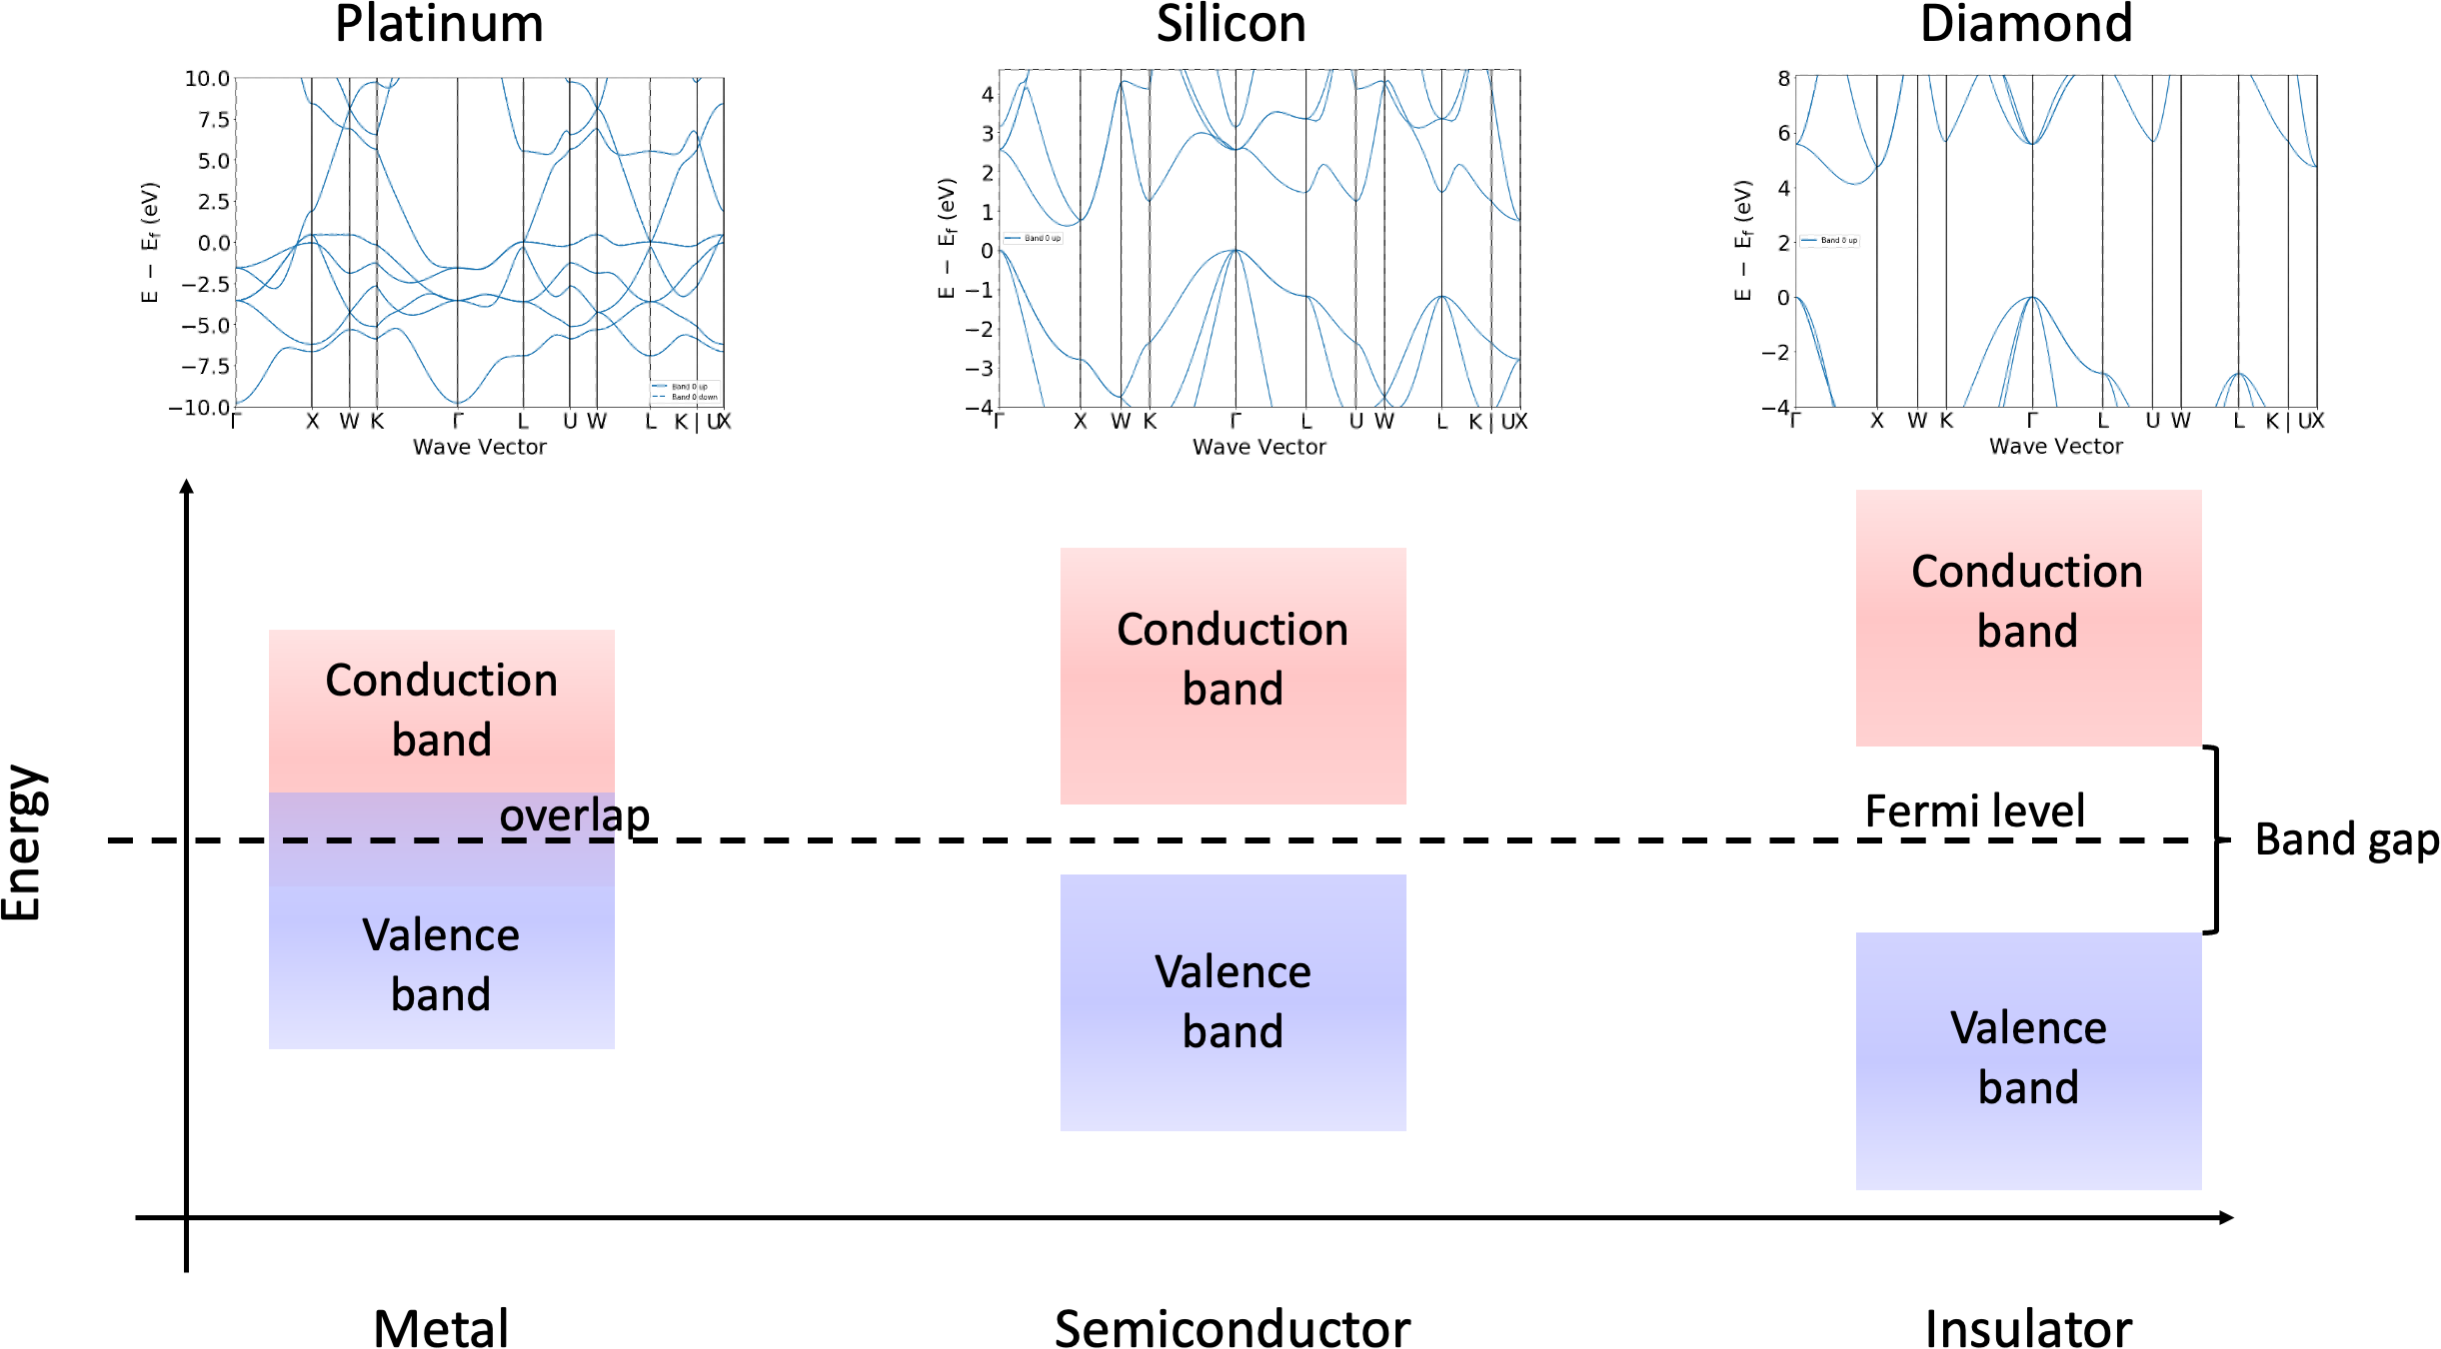
\includegraphics[width=0.8\textwidth]{Figures/DummyBandGap1_crop.png}
%    \caption{I know this is not what the paper requires here!!!}
%    \label{fig:dummyEBS}
%\end{figure}

\begin{figure}[H]
    \centering
        \subfigure[]{
        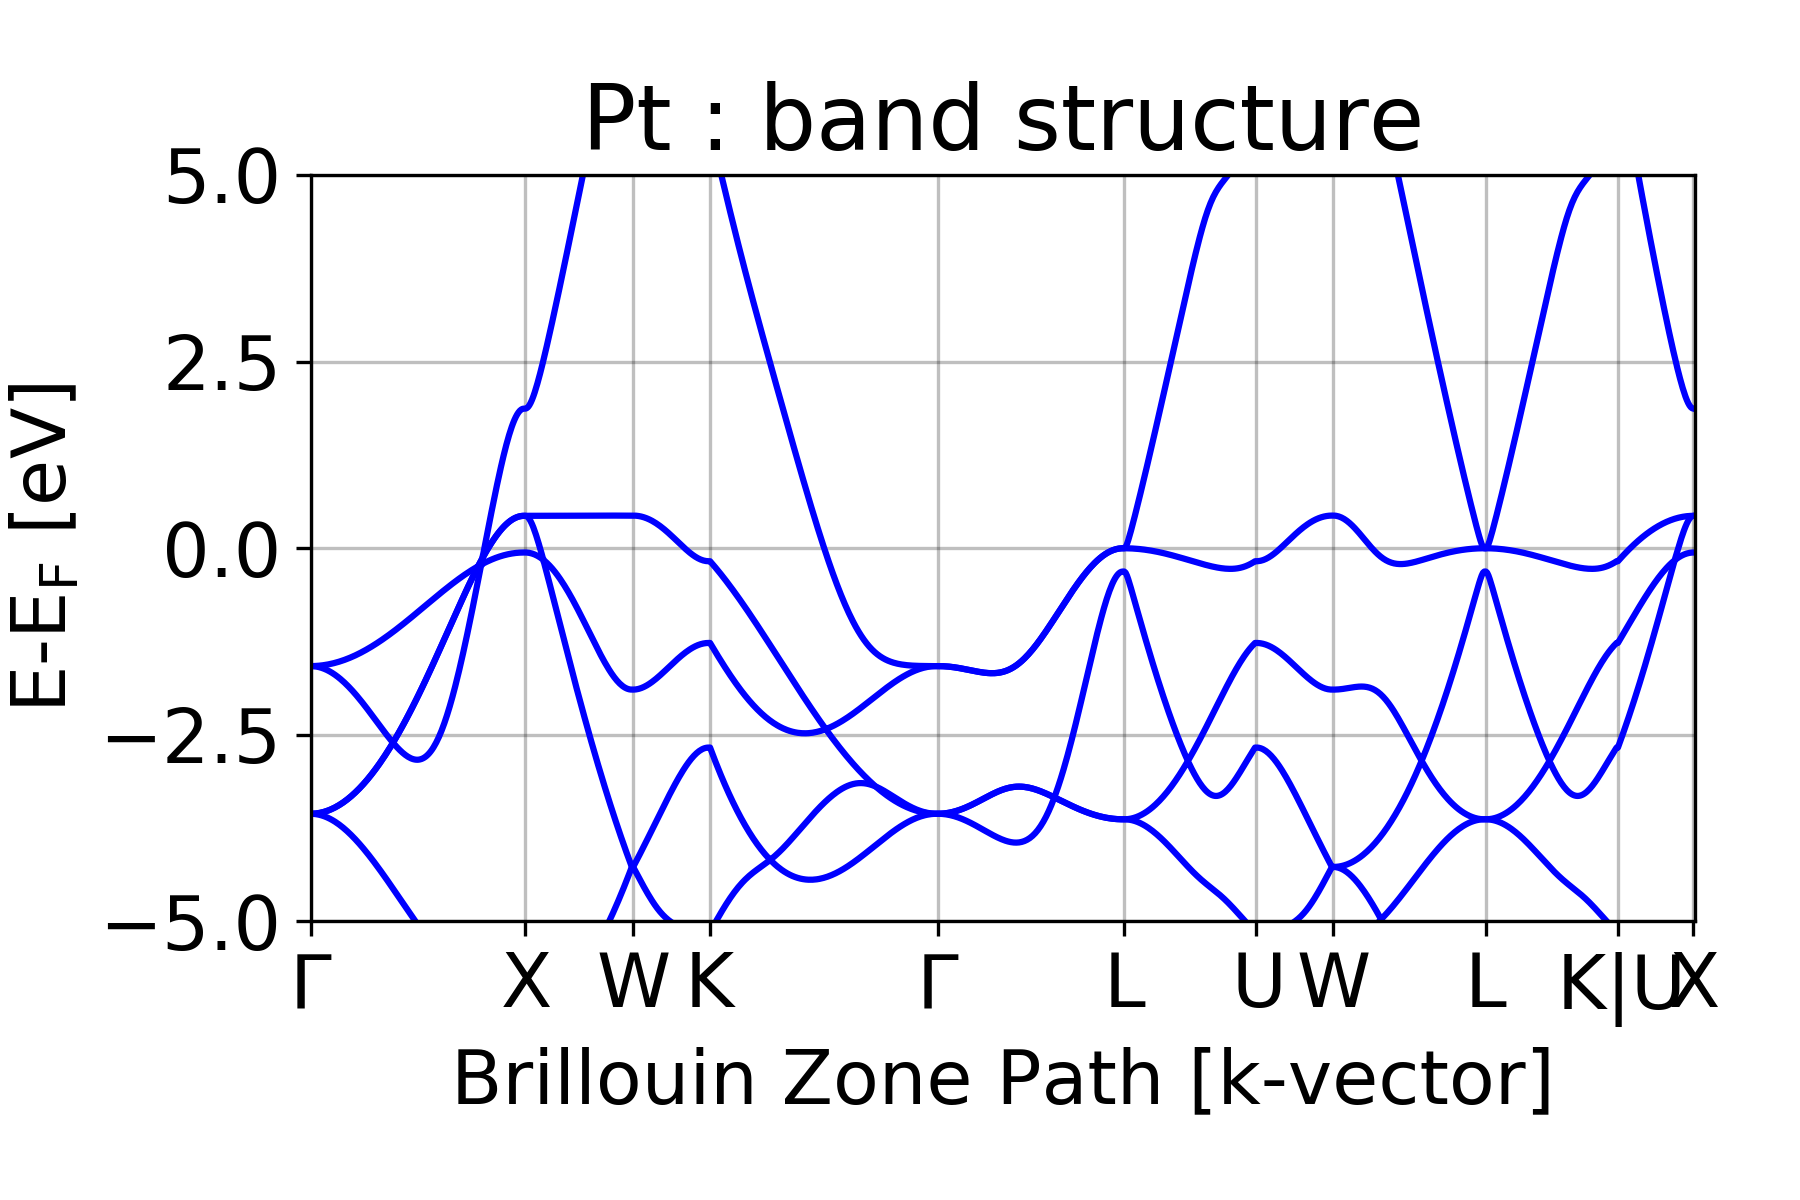
\includegraphics[width=3.0in]{Figures/mp-126_band-structure.png}
        \label{fig:Pt_EBS}
        }
        %\quad
        
        \subfigure[]{
        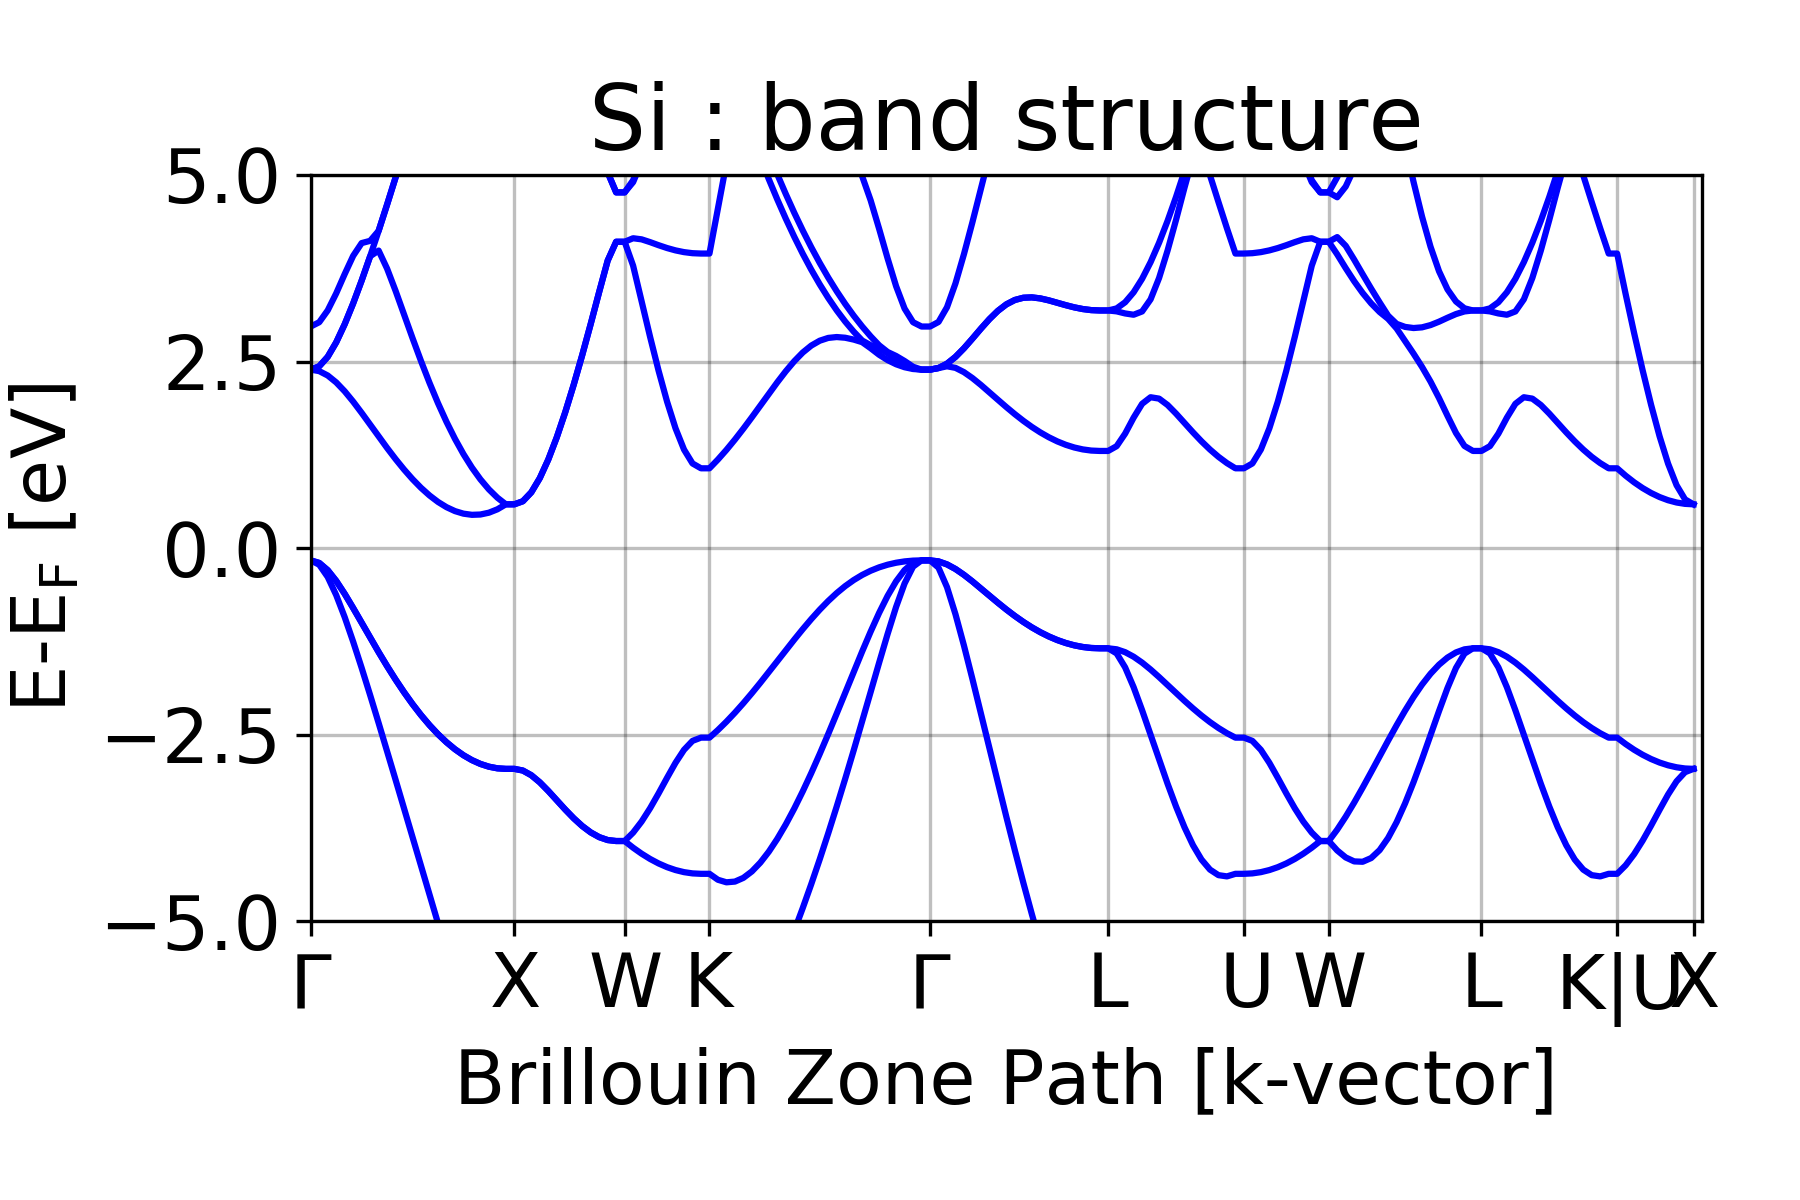
\includegraphics[width=3.0in]{Figures/mp-149_band-structure.png}
        \label{fig:Si_EBS}
        }
        %\quad
        
        \subfigure[]{
        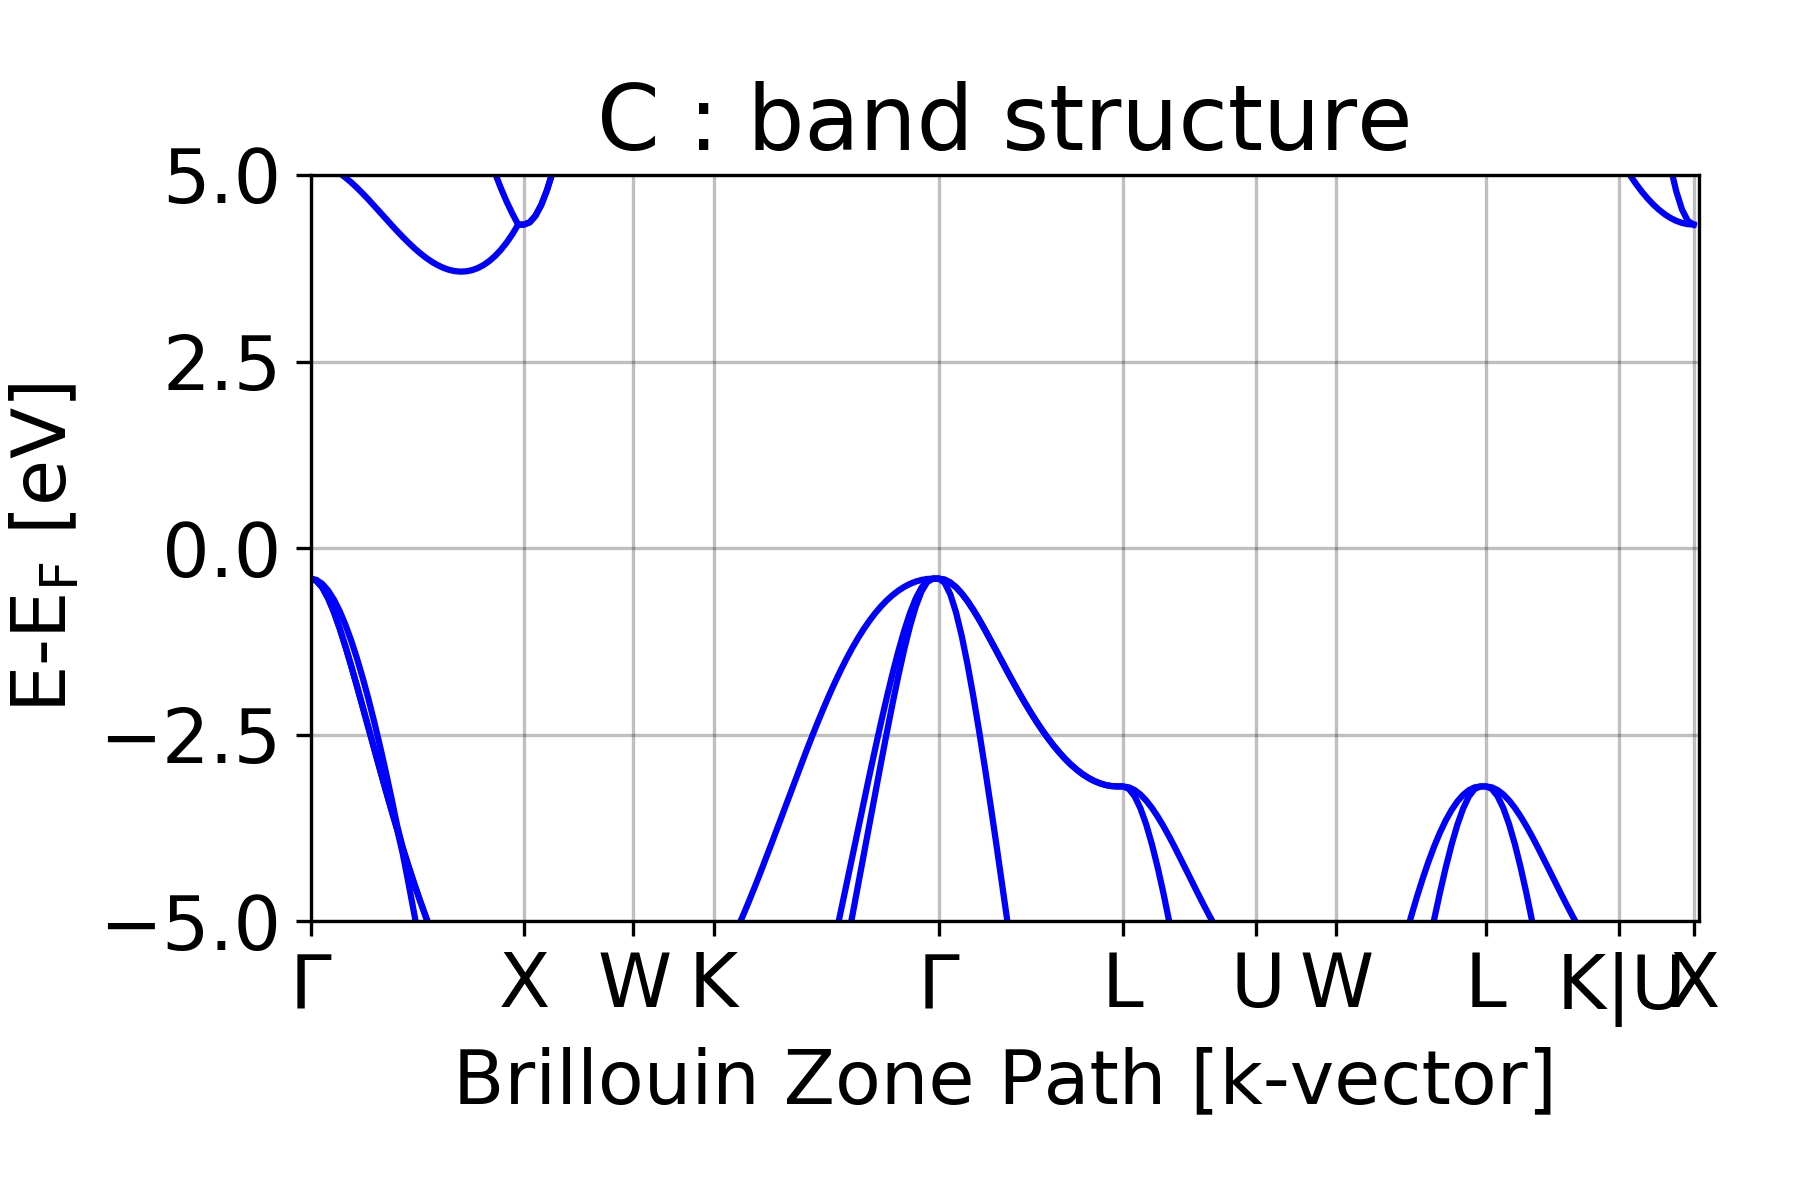
\includegraphics[width=3.0in]{Figures/mp-66_band-structure.png}
        \label{fig:Diamond_EBS}
        }
    \caption{comparison of EBSs for metallic vs semiconducting vs insulating behavior using: a) metallic (\ch{Pt}), b) semiconducting (\ch{Si}), and c) insulating (Diamond). The energies of the band gaps are \SI{4.34}{\electronvolt} for Diamond,  \SI{0.85}{\electronvolt} for \ch{Si} and \SI{0.0}{\electronvolt} for \ch{Pt}. These EBSs were taken from Materials Project (MP) database \cite{Jain2013,jain2013commentary,ong2015materials} their MP-id are included in the legend of each material. [colors online]}
    \label{fig:EBS_classical}
\end{figure}

\begin{figure}[H]
    \centering
    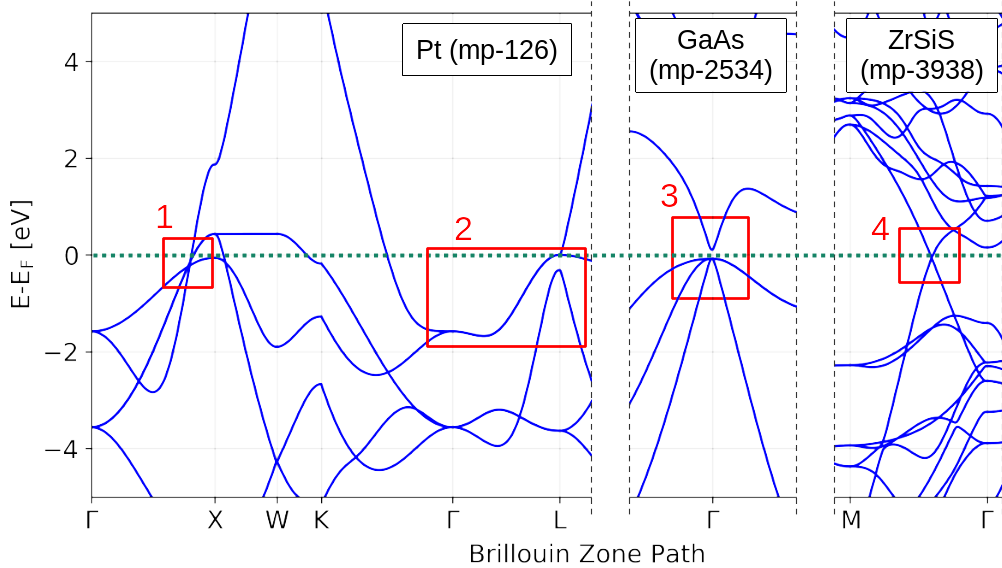
\includegraphics[width=0.7\textwidth]{Figures/band-structure-features.png}
    \caption{Deeper patterns in the EBS for Platinum (\ch{Pt}), Gallium arsenide (\ch{GaAs}), and Zirconium Silicon Sulfide (\ch{ZrSiS}). Red boxes correspond to 1. tilted Dirac point, 2. Nodal line, 3. local flat band with other highly dispersive bands, and 4. Dirac point at the Fermi level. The EBSs were taken from Materials Project (MP) database,\cite{Jain2013} their MP-id are included in the legend of each material. [colors online]}
    \label{fig:EBS_deeper_patterns}
\end{figure}

Currently, electronic band structures are calculated using Density Functional Theory (DFT), a powerful method for quantum mechanical calculations of many body systems. While successful at generating accurate results for nonmagnetic and low spin-orbit coupled systems, DFT calculations become computationally expensive as non-idealities of the model are considered. This includes crystals defects, magnetism, strong spin-orbit coupling (SOC), large unit cells, strong electron correlation (J), etc. It is also time consuming to carry out these calculations en-masse; while the Materials Project\cite{ward2018matminer} has approximately 100K materials in the database, this is a small number compared to the more than \num{d18} possible material combinations predicted to exist, and carrying out full DFT + SOC + U + magnetism calculations on that dataset is simply unrealistic. While supercomputers and new exchange-correlation functional development aid in expanding the reach of DFT, another compelling approach may be to use artificial intelligence (AI) algorithms---such as machine learning (ML)---to predict patterns in EBSs from a chemical composition and crystal structure without carrying out intensive DFT calculations. Thus, by training on known DFT computed EBSs and learning what chemical compositions/structural features drive certain electronic structure patterns, it is possible to use AI models as a rapid screening tool and identify promising material classes or candidates for deeper theoretical and experimental investigation as well as to discover new materials with desired properties. These machine learning methods center around the core idea of learning against the hidden correlations of the material's structures with the physical property of relevance for a subgroup of materials, where the property values are either computationally computed or experimentally available, to quantitatively establish a structure-property relationship. The insight gained from the subgroup of materials is then utilized to deliver predictions on the property for all materials in the parent group, thus eliminating the need for spending time consuming computational or experimental resources for these structures.\cite{moghadam2019structure,sun2019machine,zhou2019big,goldsmith2018machine,toyao2019machine} In the case where there is a paucity of experimental physical property data but a particular pattern in the electronic band structure is known to relate to a physical property of interest, the correlation methodology can become focused on learning against the correlations of the material's structure with the electronic band structure. This approach has precedence, being used in prediction of novel thermoelectrics,\cite{JiaXue2022,NaGyoungS2021,ShengYe2020} construction materials,\cite{MASOODCHAUDRY2021101897} solar cell materials,\cite{ChoudharyKamal2019,doi:10.1021/acs.jpclett.1c03526} and more. 

%\textcolor{red}{What are the limitations for the DFT based calculation works}
%\textcolor{red}{Include a paragraph narrowing down to the Heuslers---why Heuslers among all QM materials?\\
%Heusler applications: topological isolators - Dirac and Weyl semimetals - Magnetic thin film\\
%Among QM Materials, comprise by \textcolor{red}{names and formula list}---the Heuslers ``Family'' highlight by their \textcolor{red}{list of attributes that make Heuslers better candidates}. Regarding Heuslers EBS bla bla bla.}

To begin this approach for QMs, first we narrow our materials of interest to a particularly successful class of QM materials, the Heusler family,\cite{galanakis2016theory,graf2010heusler,casper2012half,graf2011simple,poon2018recent,chibani2018first} which has attracted major interest from the community for their wide-ranging applications in the domain of spintronics,\cite{birsan2020zr,khandy2019full,casper2012half} thermoelectrics,\cite{zaferani2019strategies,poon2018recent,chibani2018first} superconductors,\cite{hu2021charge,xiao2018superconductivity,uzunok2020physical,kautzsch2019aupdtm} solar-cells,\cite{abdel2021high,murtaza2021lead,wang2020photoactive,leoncini2022correlating} multifunctional topological insulators,\cite{sattigeri2021dimensional,barman2018topological,zhang2020machine} etc. Chemically, they are ternary compounds which can be further distinguished into ``half'' and ``full'' Heuslers based on their stoichiometry. The chemical formula for half-Heuslers and full-Heuslers are of the form \ch{XYZ} (1:1:1) and \ch{X2YZ} (2:1:1) respectively, where \ch{X} and \ch{Y} generally have a cationic character (\textit{d}-block elements--transition metals) and Z is expected to be the anionic counterpart (\textit{p}-block elements). Crystallographically, Heusler compounds exhibit a face-centered cubic crystal structure, as depicted on Figure \ref{fig:HeuslersCrystalStructure}, with space groups \num{216} and \num{225} for half-Heuslers and full-Heuslers respectively. As a myriad of chemical choices are possible with the X, Y and Z sites, Heusler's material properties can be tuned by altering the composition, which can be leveraged for accelerating material development in applications.

\begin{figure}[H]
    \centering
    %\subfigure[]{
    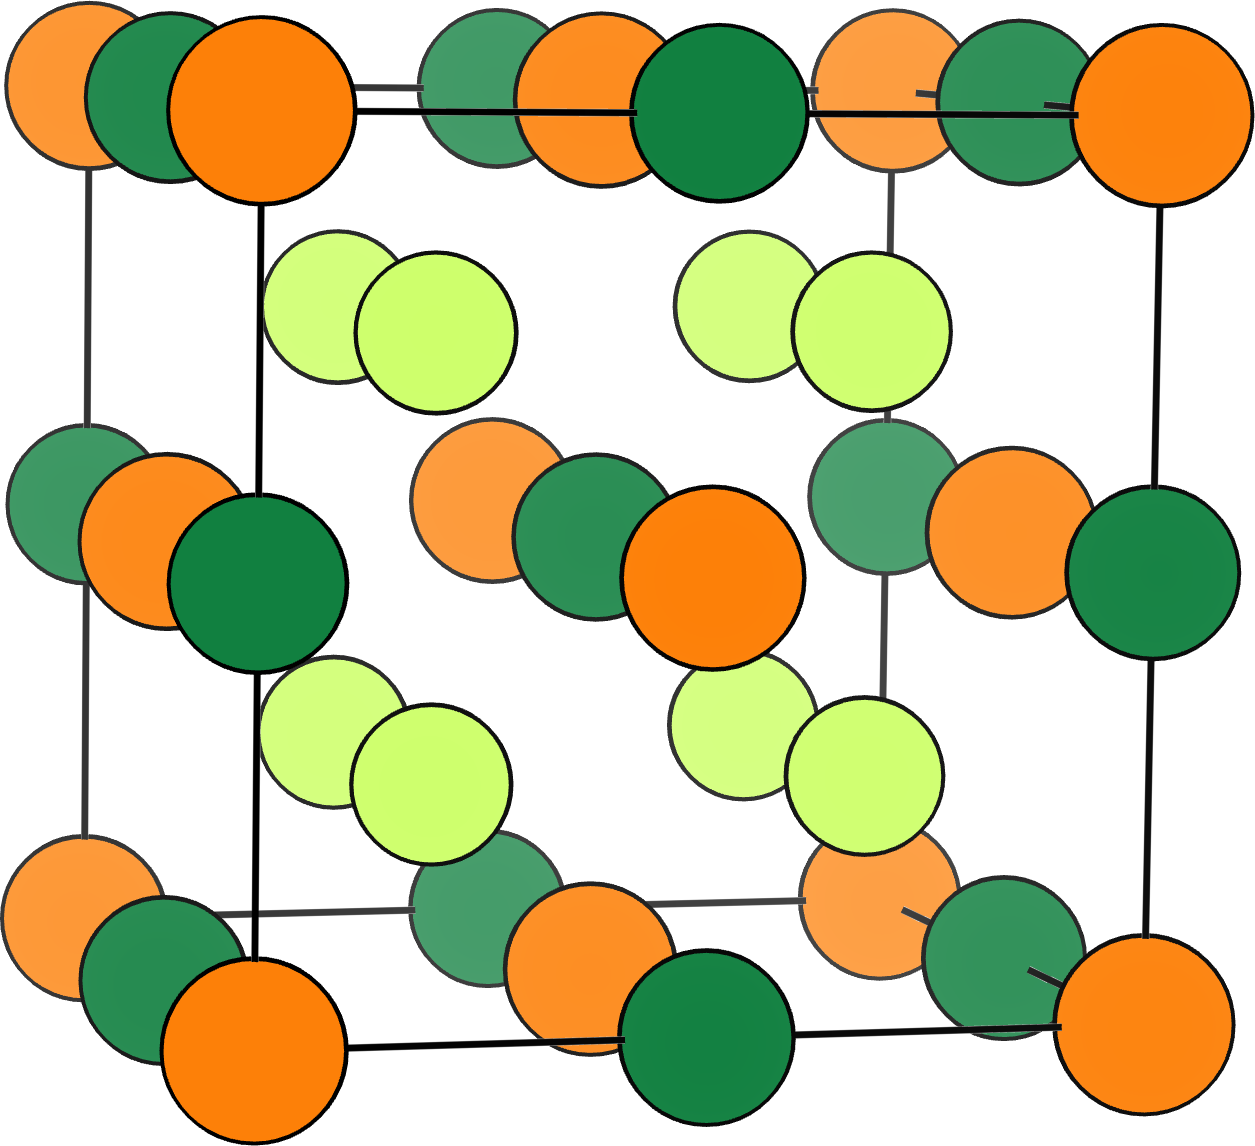
\includegraphics[scale=0.30]{Figures/MnAlCu2.png}
    %\label{fig:Heuslers}
    %}
    %\quad
    %\subfigure[]{
    %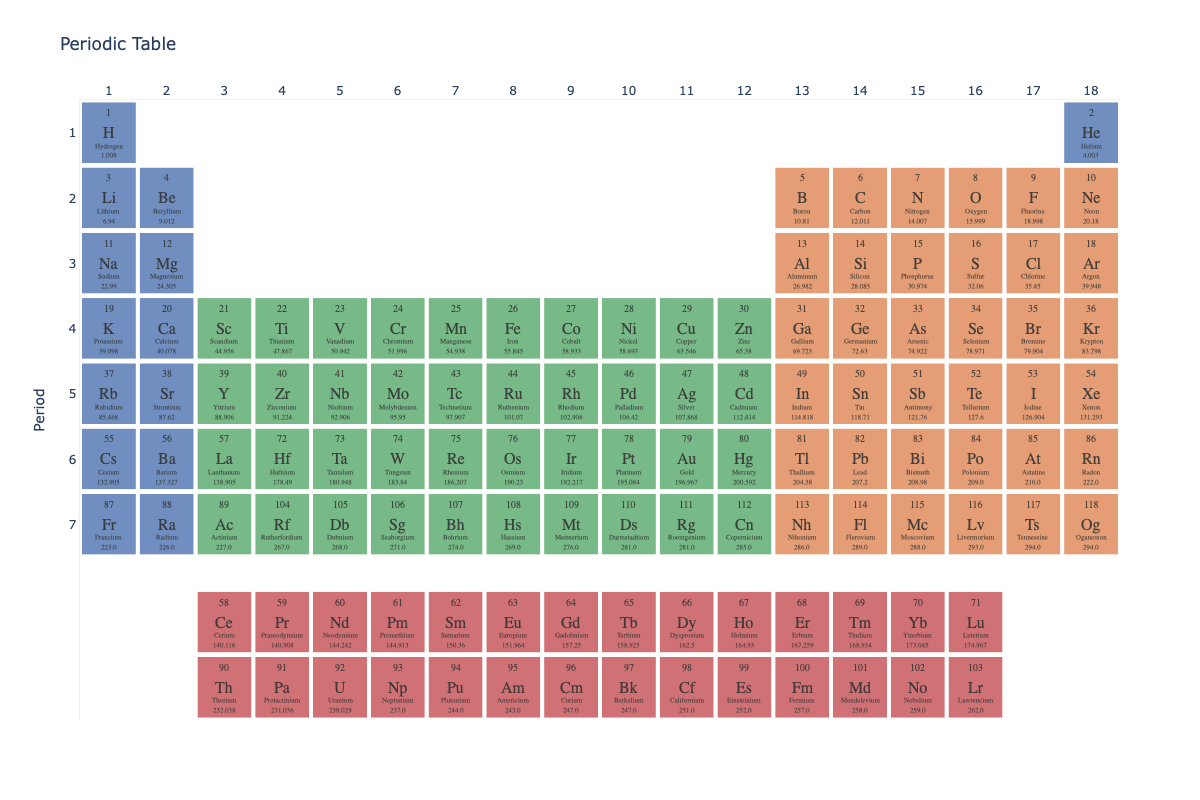
\includegraphics[scale=0.15]{Figures/PeriodicTablebyBlocks.png}
    %\label{fig:HeuslersPeriodicTable}
    %}
    \caption{Illustrative full-Heusler crystal---\ch{MnCu2Al} \ch{Al}, \ch{Mn}, and \ch{Cu} are colored in orange, green, and lime respectively. Structure taken from Materials Project\cite{Jain2013} (MP-id: mp-3574). [colors online]
    %; b) periodic table colored by blocks, highlighting \textit{s}, \textit{p}, \textit{d}, and \textit{f} blocks of elements in blue, orange, green, and red respectively. [colors online]
    }
    \label{fig:HeuslersCrystalStructure}
\end{figure}

The chemical composition to EBS dependency for Heuslers is, however, a complicated relationship, being dependent on which atoms are located at which atomic site in the crystal structure and the resulting interaction of their atomic orbitals.\cite{ojala2010permutation,ma2017computational,ma2018computational} %Crystallographically, Heusler compounds exhibit face-centered cubic crystal structure, as depicted on Figure \ref{fig:HeuslersCrystalStructure}. Their chemical composition can be represent by the general formulas \ch{XYZ} (half-Heuslers--space group 216) or \ch{X2YZ} (full-Heuslers--space group 225), being \ch{X} and \ch{Y} transition metal elements, whereas \ch{Z} is a \textit{p}-block element. 
A challenge in Heusler design is to predict how the chemical composition and crystallographic arrangement influences EBSs without requiring exhaustive DFT calculation. However, given the large number of possibilities, comprising $>$ \num{1500} known members with an exponentially larger number of possibilities if different atomic crystal arrangements are considered for a given composition, first-principles calculation and learning of their influence on the EBS is unmanageable, making it a good test bed for attempting to use AI and ML as mentioned above.
%Another approach, a material informatics approach, has become in the last decade an attractive alternative due to the following advantages: 1) access to chemical, crystal structure, and EBS databases, and 2) avoiding the need of performing intensive DFT calculations to compute the EBS. By using a convenient artificial intelligent (AI) algorithm---e.g., machine learning (ML) or graphical neural networks (GCC)---a composition/EBS relationship can be developed. 
%By performing data mining within available materials databases, and identifying a set of relevant features that would be able to describe patterns in EBS based on a chemical composition and/or atomic crystal arrangement without carrying out intensive DFT calculations using  machine learning (ML) algorithms. Thus, predicting patterns in EBS based on a chemical composition and/or structural formula without carrying out intensive DFT calculations.

%Specifically, by training AI models on known DFT computed EBSs (from freely available databases) and learning what chemical compositions/structural features drive certain electronic structure patterns, we can use AI models as a rapid screening tool to identify promising material candidates for deeper theoretical and experimental investigation.

%Finding optimal candidate materials for any given application can be intensely time expensive due to vast scope of structures that are available, this hindrance further gets compounded by the high dimensionsionality each structure offers when the substitutions are conducted within the base formula. Such factors combinatorically explode the search region which further boils down to substantially increased screening time per structure. Computational techniques involving first principles methods such as DFT (Density Functional Theory) can speed up the material screening process but not substantial enough to achieve material discovery under a reasonable time. 

%Such sophisticated learning approaches can make thorough inroads in delivering insights which guide our understanding of the underlying correlations of a material structure and a desired property. %this enables us to rapidly accelerate the material discovery process by heavily cutting short the screening process per structure and leads us closer to the candidate materials in a fairly reasonable time-frame. 

%Here we begin this approach by attempting to use AI+ML in a targeted fashion; to recognize Dirac points within a specific range of the ground state energy in the blah blah blah. Cubic materials, Heuslers, why these limitations were chosen, Dirac points were identified using AI algorithms, then ML training was carried out, what we saw/learned (summary).
We create a Heuslers dataset using the Materials Project (MP) database;\cite{Jain2013} considering compounds with cubic crystal structures and general formulas \ch{XYZ} and \ch{X2YZ}, which correspond to space groups 216 and 225 (a total \num{276} compounds). The EBSs are also retrieved from the MP which are computed using DFT calculations. Using this Heuslers dataset along with the python library Matminer\cite{WARD201860, Matminer} for rapid features extraction, we developed an ML model that correlates Heusler's chemical compositions with their EBSs; specifically with the number of band crossings within a specific range of the ground state energy ($\pm$\SI{1}{\electronvolt}). We extract the number of crossings from the EBS using an automated algorithm to mine the EBS for that particular pattern. The ML model is then developed using the XGBoost algorithm\cite{chen2016xgboost,chen2015xgboost}---a parallel tree boosting technique under Gradient Boosting framework---to train the model as a function of periodic table properties of the materials constituent elements (chemical composition) and global crystal structure parameters. Also, since the Heuslers dataset consists of a relatively small number of compounds (\num{276}), we also created a dataset of cubic compounds removing the restriction of specific transition metal atoms for \ch{X} and \ch{Y} elements, and \textit{p}-block atoms for \ch{Z} elements, but retaining the space groups \num{216} and \num{225}. This ``Cubic dataset'' consists of \num{3751} structures, and is used to benchmark the ML models and understand the generalizability of the insight gained from the Heuslers dataset.
%and by using ML, train a prediction model correlating composition-EBS. Our ML model recognize Dirac points within a specific range of the ground state energy in the blah blah blah. We consider materials with the general formulas \ch{XYZ} and \ch{X2YZ}. Creating a database of \textcolor{red}{$\mathrm{\geq}$ \SI{200}{K}} structures, database features + where could be access (paying). The electronic band structure, in the database, are taken from XXX, which were computed using DFT calculations. Using \textcolor{red}{database name} along with python module matminer, for rapid features extraction, we present a ML model correlating the \textcolor{red}{Heuslers} chemical composition with the electronic band structure number of crossing (within $\pm$\SI{1}{\electronvolt}). Specifically, we use the XGBoost algorithm---a parallel tree boosting technique under Gradient Boosting framework---to develop the ML model, which is a function of periodic table properties of the materials constituent elements (chemical composition). Making the model feasible to use for anyone with an internet connection.

\section{Methodology}
%The author names and affiliations could be formatted in two ways:
%\begin{enumerate}[(1)]
%\item Group the authors per affiliation.
%\item Use footnotes to indicate the affiliations.
%\end{enumerate}
%See the front matter of this document for examples. You are recommended to conform your choice to the journal you are submitting to.

\subsection{Materials Data-set}
The data used in this work is entirely sourced from the the Materials Project with $\sim$ \num{76240} entries of EBSs calculated via DFT. %Other reputable EBS databases are also freely available like the \href{https://www.topologicalquantumchemistry.com/#/}{Topological Materials Database (TMD)}, the \href{http://materiae.iphy.ac.cn/}{Material Sciences Database (MTR)}, the \href{https://jarvis.nist.gov/login?next=/jarvisdft/}{JARVIS DFT dataset} or the \href{https://omdb.mathub.io/}{Organic Materials Database (OMDB)}. While each database exhibits at least one compelling advantage with respect to the others, we find that the resolution (i.e. smoothness of the EBS traces) and wide choice of materials of the MP dataset was more suitable for the type of processing that we applied. The choice of the starting data source was also influenced by the ease of accessibility (i.e. availability and documentation of APIs, presence of numerical data vs picture data, presence of request or bandwidth limitations), the type of compounds present (our focus is not on organic materials) as well as the transparency of the data provided by the databases.
For the Heusler and Cubic dataset with space groups of \numlist{216;225}, the whole MP database was searched---using the pymatgen python library\cite{ONG2013314}---for materials with cubic crystal symmetry (space groups \numlist{216;225}) which were then downloaded including their chemical, structural, EBS. The total number of materials found after this search was \numlist{276;3751} for the Heuslers and Cubic datasets respectively; and are available at \href{https://github.com/Material-Mind/Heuslers-EBS-Dirac-points.git}{GitHub Link}. Heuslers dataset is formed by \numlist{107;169} half (space group 216) and full (space group 225) Heuslers respectively. Consisting of compounds comprised by \ch{X} and \ch{Y} elements from groups \numrange{1}{12} (\textit{s} and \textit{d} blocks) and periods \numrange{4}{6}; and \ch{Z} elements from groups \numrange{13}{16} and (\textit{p}-block) periods \numrange{3}{6} (see Figure \ref{fig:small_dataset_compo}). On the other hand, the Cubic dataset consist of compounds comprised by \ch{X} and \ch{Y} elements from groups \numrange{1}{12} (\textit{s} and \textit{d} blocks) and periods \numrange{1}{6}; and \ch{Z} elements from groups \numrange{13}{17} (\textit{p}-block) and periods \numrange{2}{6} (see Figure \ref{fig:big_dataset_compo}). The Heuslers dataset compounds are constrained to have for \ch{X} and \ch{Y} elements \textit{s} and \textit{d} blocks atoms whereas for \ch{Z} element \textit{p}-block atoms. These constraints are removed for the Cubic dataset compounds i.e. \ch{X}, \ch{Y}, and \ch{Z} can be either \textit{s}, \textit{d} or \textit{p}-block elements. However, the symmetry constraints (space groups 216 or 225) were retained. Noteworthy, \ch{X}, \ch{Y} and \ch{Z} elements in the Cubic dataset exhibit counting ranging from $\sim$\numrange{75}{225}, highlighting fluorine (\ch{F}) with an outlier counting of \num{450}. In contrast, \ch{X}, \ch{Y} and \ch{Z} elements in the Heuslers dataset exhibit counting ranging from $\sim$\numrange{7}{55}. 
%\textcolor{red}{This paragraph have to be rewritten for the including small dataset info} The whole MP database was searched for materials with cubic crystal symmetry (space groups \numrange{195}{230}) which were downloaded including their chemical, structural, EBS and mechanical data. The total number of materials found after this initial search was \num{20828}, and are available at \textcolor{blue}{GitHub Link}. It is critical to further restrict the symmetry group---included in the dataset for the ML model---in order to prevent the number of local feature from increasing beyond control, as the worst case scenario we want to avoid is to have fewer training data points than features. Ending up with a \num{3751} materials dataset---also available at \textcolor{blue}{GitHub Link}, which consist of compounds comprised by element from groups \numrange{1}{17} and periods \numrange{1}{6} (see Figure \ref{fig:big_dataset_compo}). \textcolor{red}{In contract, the Heuslers data set (see Figure \ref{fig:small_dataset_compo}). Mention something about the heatmaps.}

\begin{figure}[H]
    \centering
        \subfigure[]{
        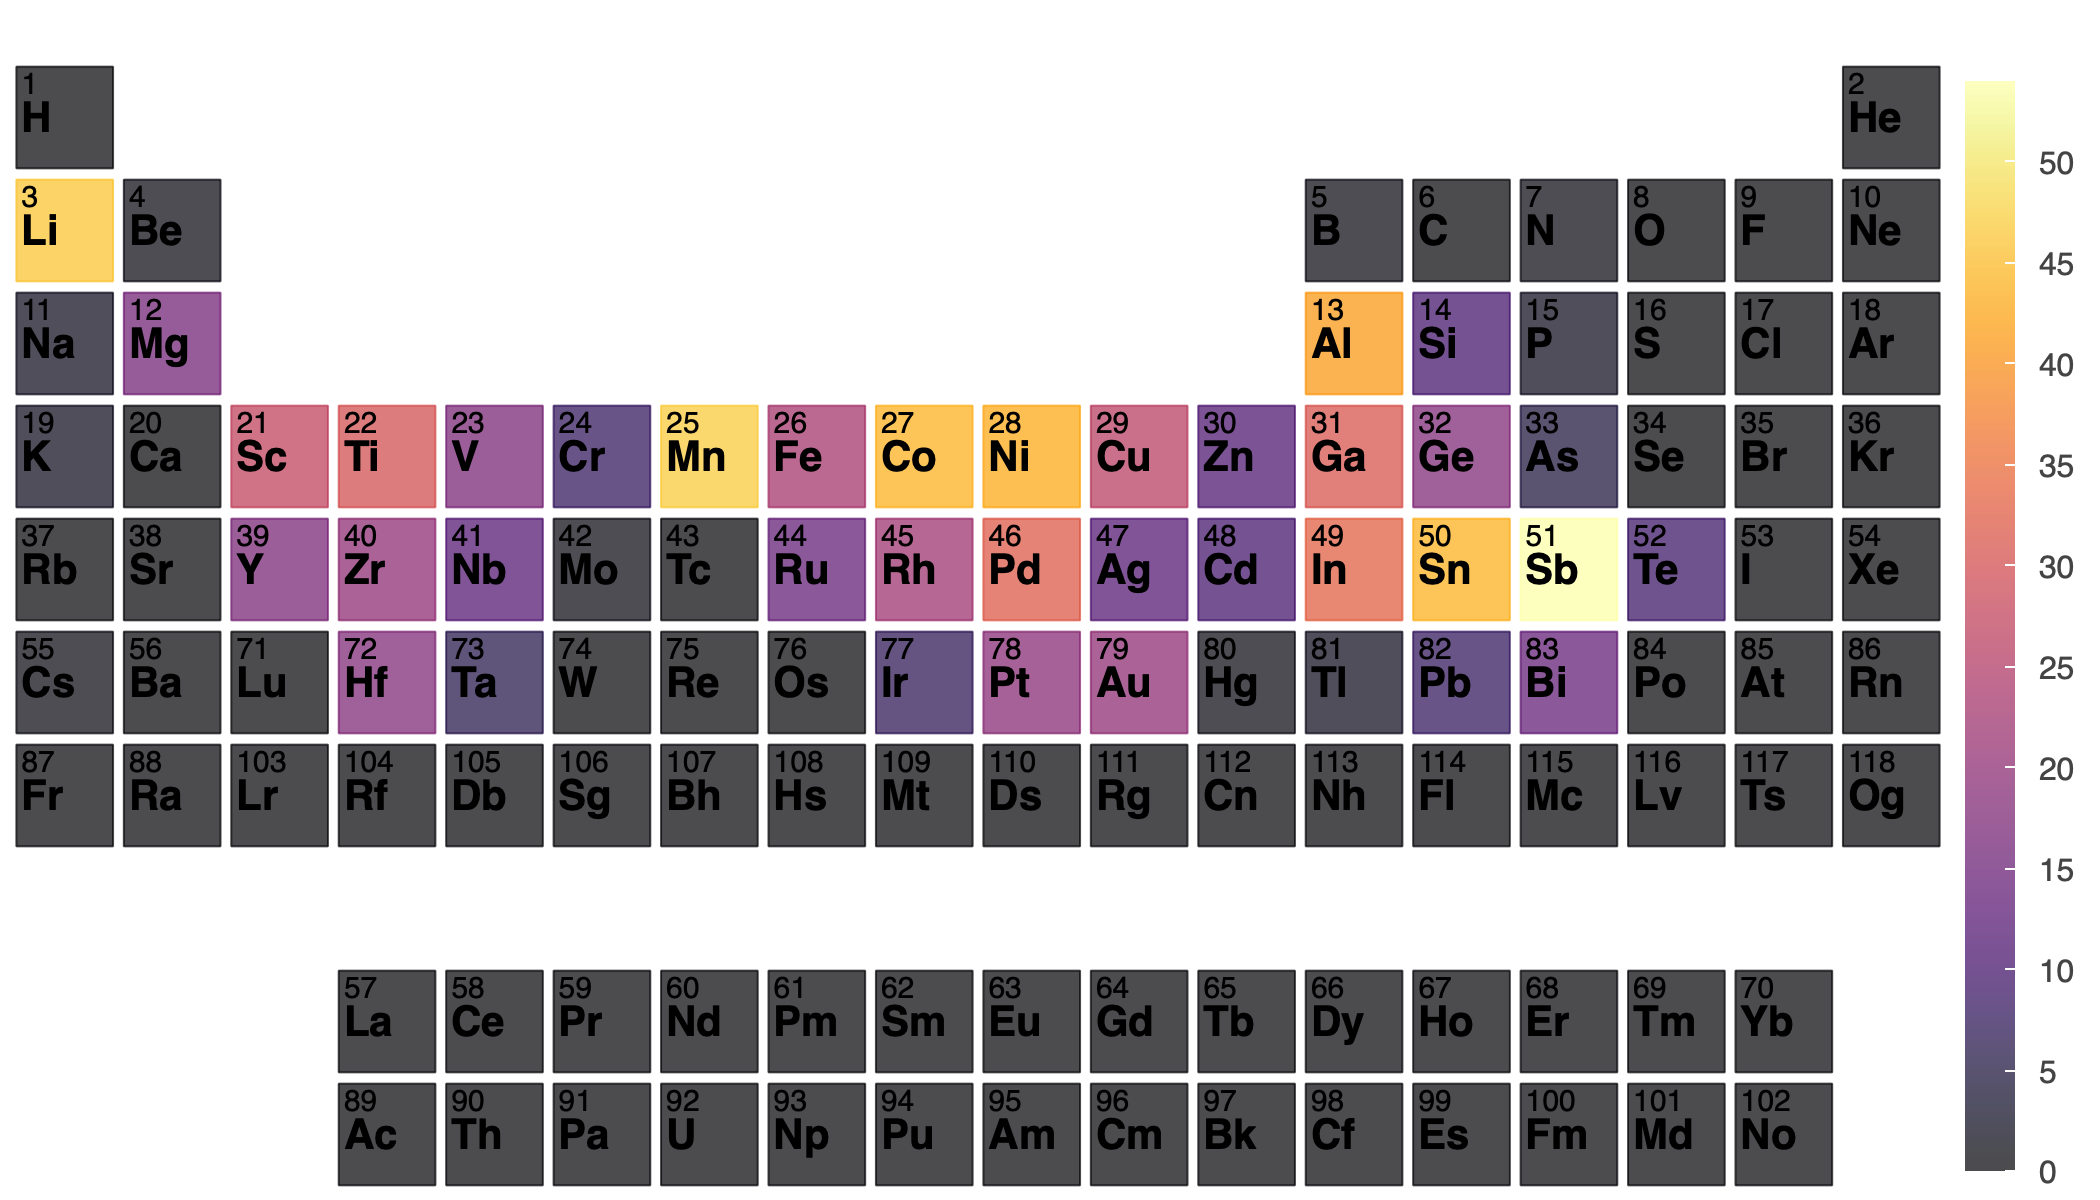
\includegraphics[width=3in]{Figures/bokeh_plot_sds.png}
        \label{fig:small_dataset_compo}
        }
        \quad
        \subfigure[]{
        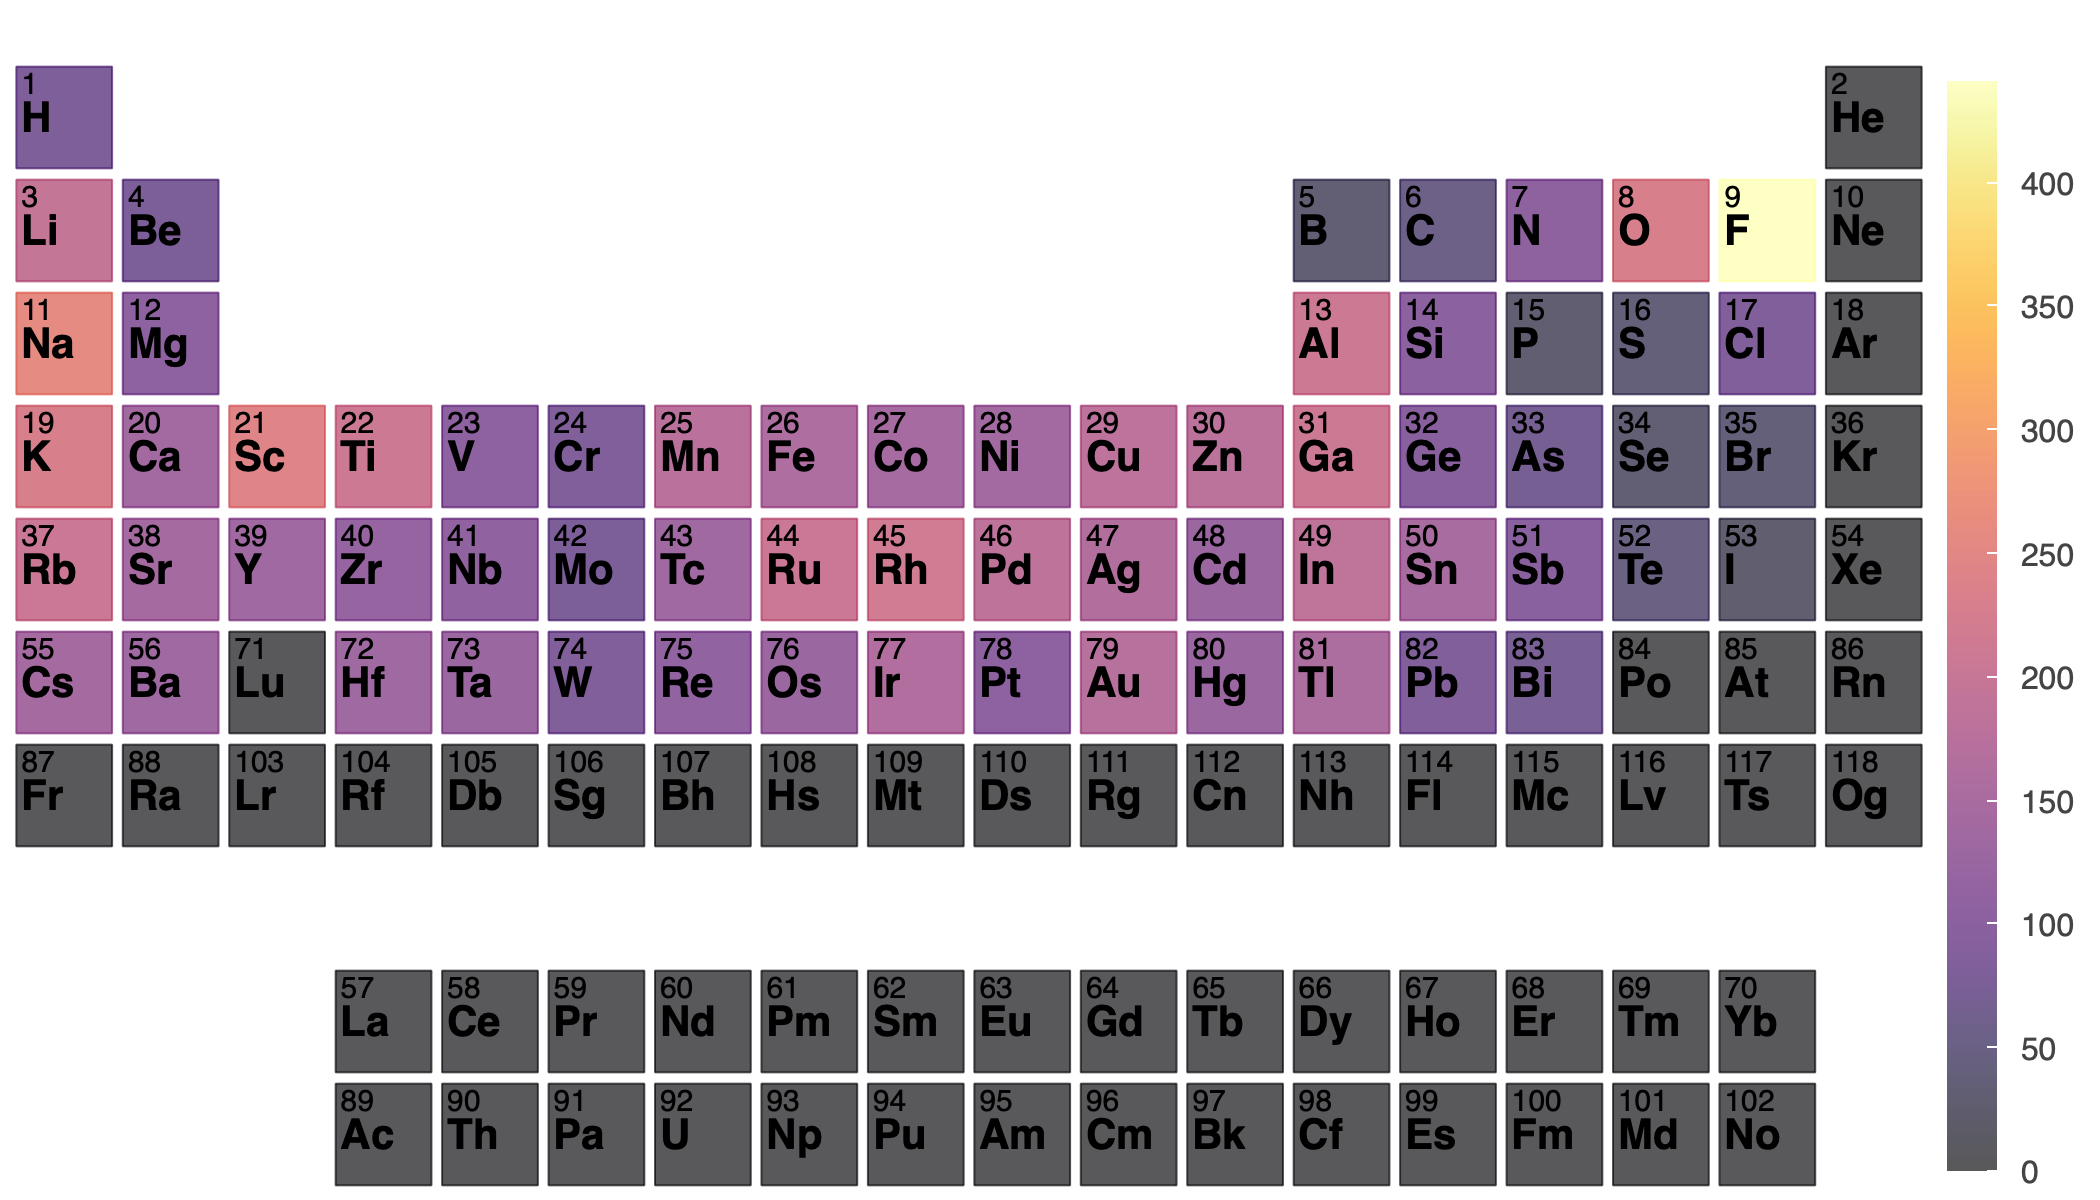
\includegraphics[width=3in]{Figures/bokeh_plot_bds.png}
        \label{fig:big_dataset_compo}
        }
\caption{a) Periodic table heatmap for element appearance on Heuslers dataset, b) Periodic table heatmap for element appearance on the Cubic dataset. Elements are colored according to their appearance on in the respective datasets, gray corresponds to no appearance and yellow for maximum appearance. [Colors online]}
\label{fig:dataset_compo}
\end{figure}

\subsection{Electronic Band Structure: Dirac points identification - Number of Crossings}
%\textcolor{teal}{Alessandro}
%\begin{figure}[H]
%    \centering
%    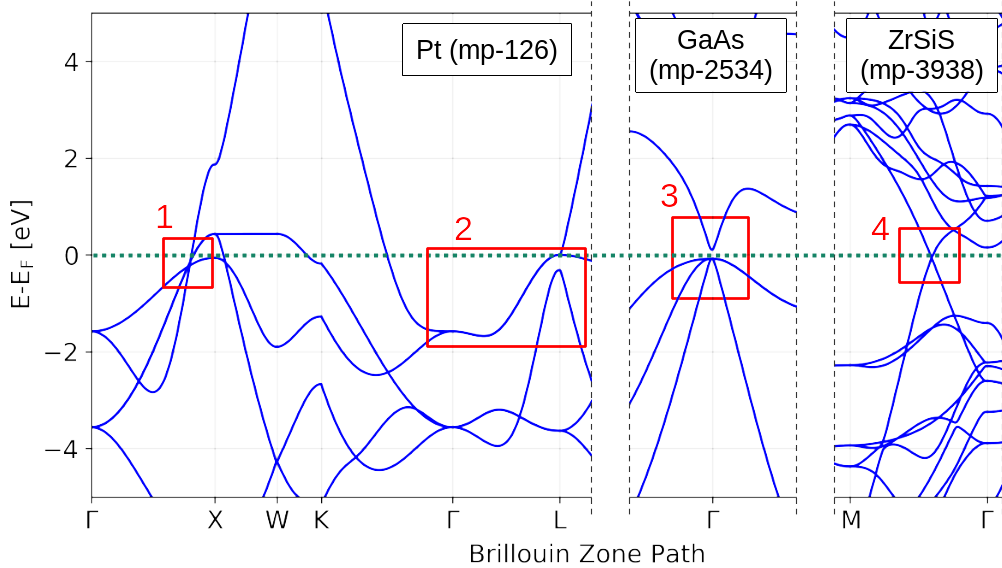
\includegraphics[width=0.7\textwidth]{Figures/band-structure-features.png}
%    \caption{Examples of features demonstrated on the EBS of cubic Pt (spacegroup 225)}
%    \label{fig:bandfeatures}
%\end{figure}
EBSs are imported as a $N \cdot K$ matrix of energy value, with N being the number of bands calculated by the DFT calculation and K being the number of momentum-points sampled along the MP-recommended BZ path. The MP database uses the BZ path convention presented in \cite{setyawan2010high}. %even though newer standards have been presented in \cite{hinuma2017band} or [ref missing].
Specifically we identify Dirac points over the EBSs---termed 'number of crossings'---within a specific range of the ground state energy ($\pm$\SI{1}{\electronvolt}). The number of crossings distributions for the Heusler and Cubic datasets are shown in Figure \ref{fig:dataset_croos}. In both cases, the distributions are right skewed but despite the Cubic dataset having \num{14} times more compounds than Heuslers dataset, both number of crossings distributions have close medians $\sim$\num{8}. Suggesting the distributions shape correspond to the number of crossings natural variation instead of an data errors or sampling problems. Also, more than \SI{50}{\percent} of the Heuslers number of crossings range consists of outlier data points (see box plot on Figure \ref{fig:small_dataset_croos}), whereas the Cubic dataset distribution has almost no outliers (see box plot on Figure \ref{fig:big_dataset_croos}).

\begin{figure}[H]
        \subfigure[]{
        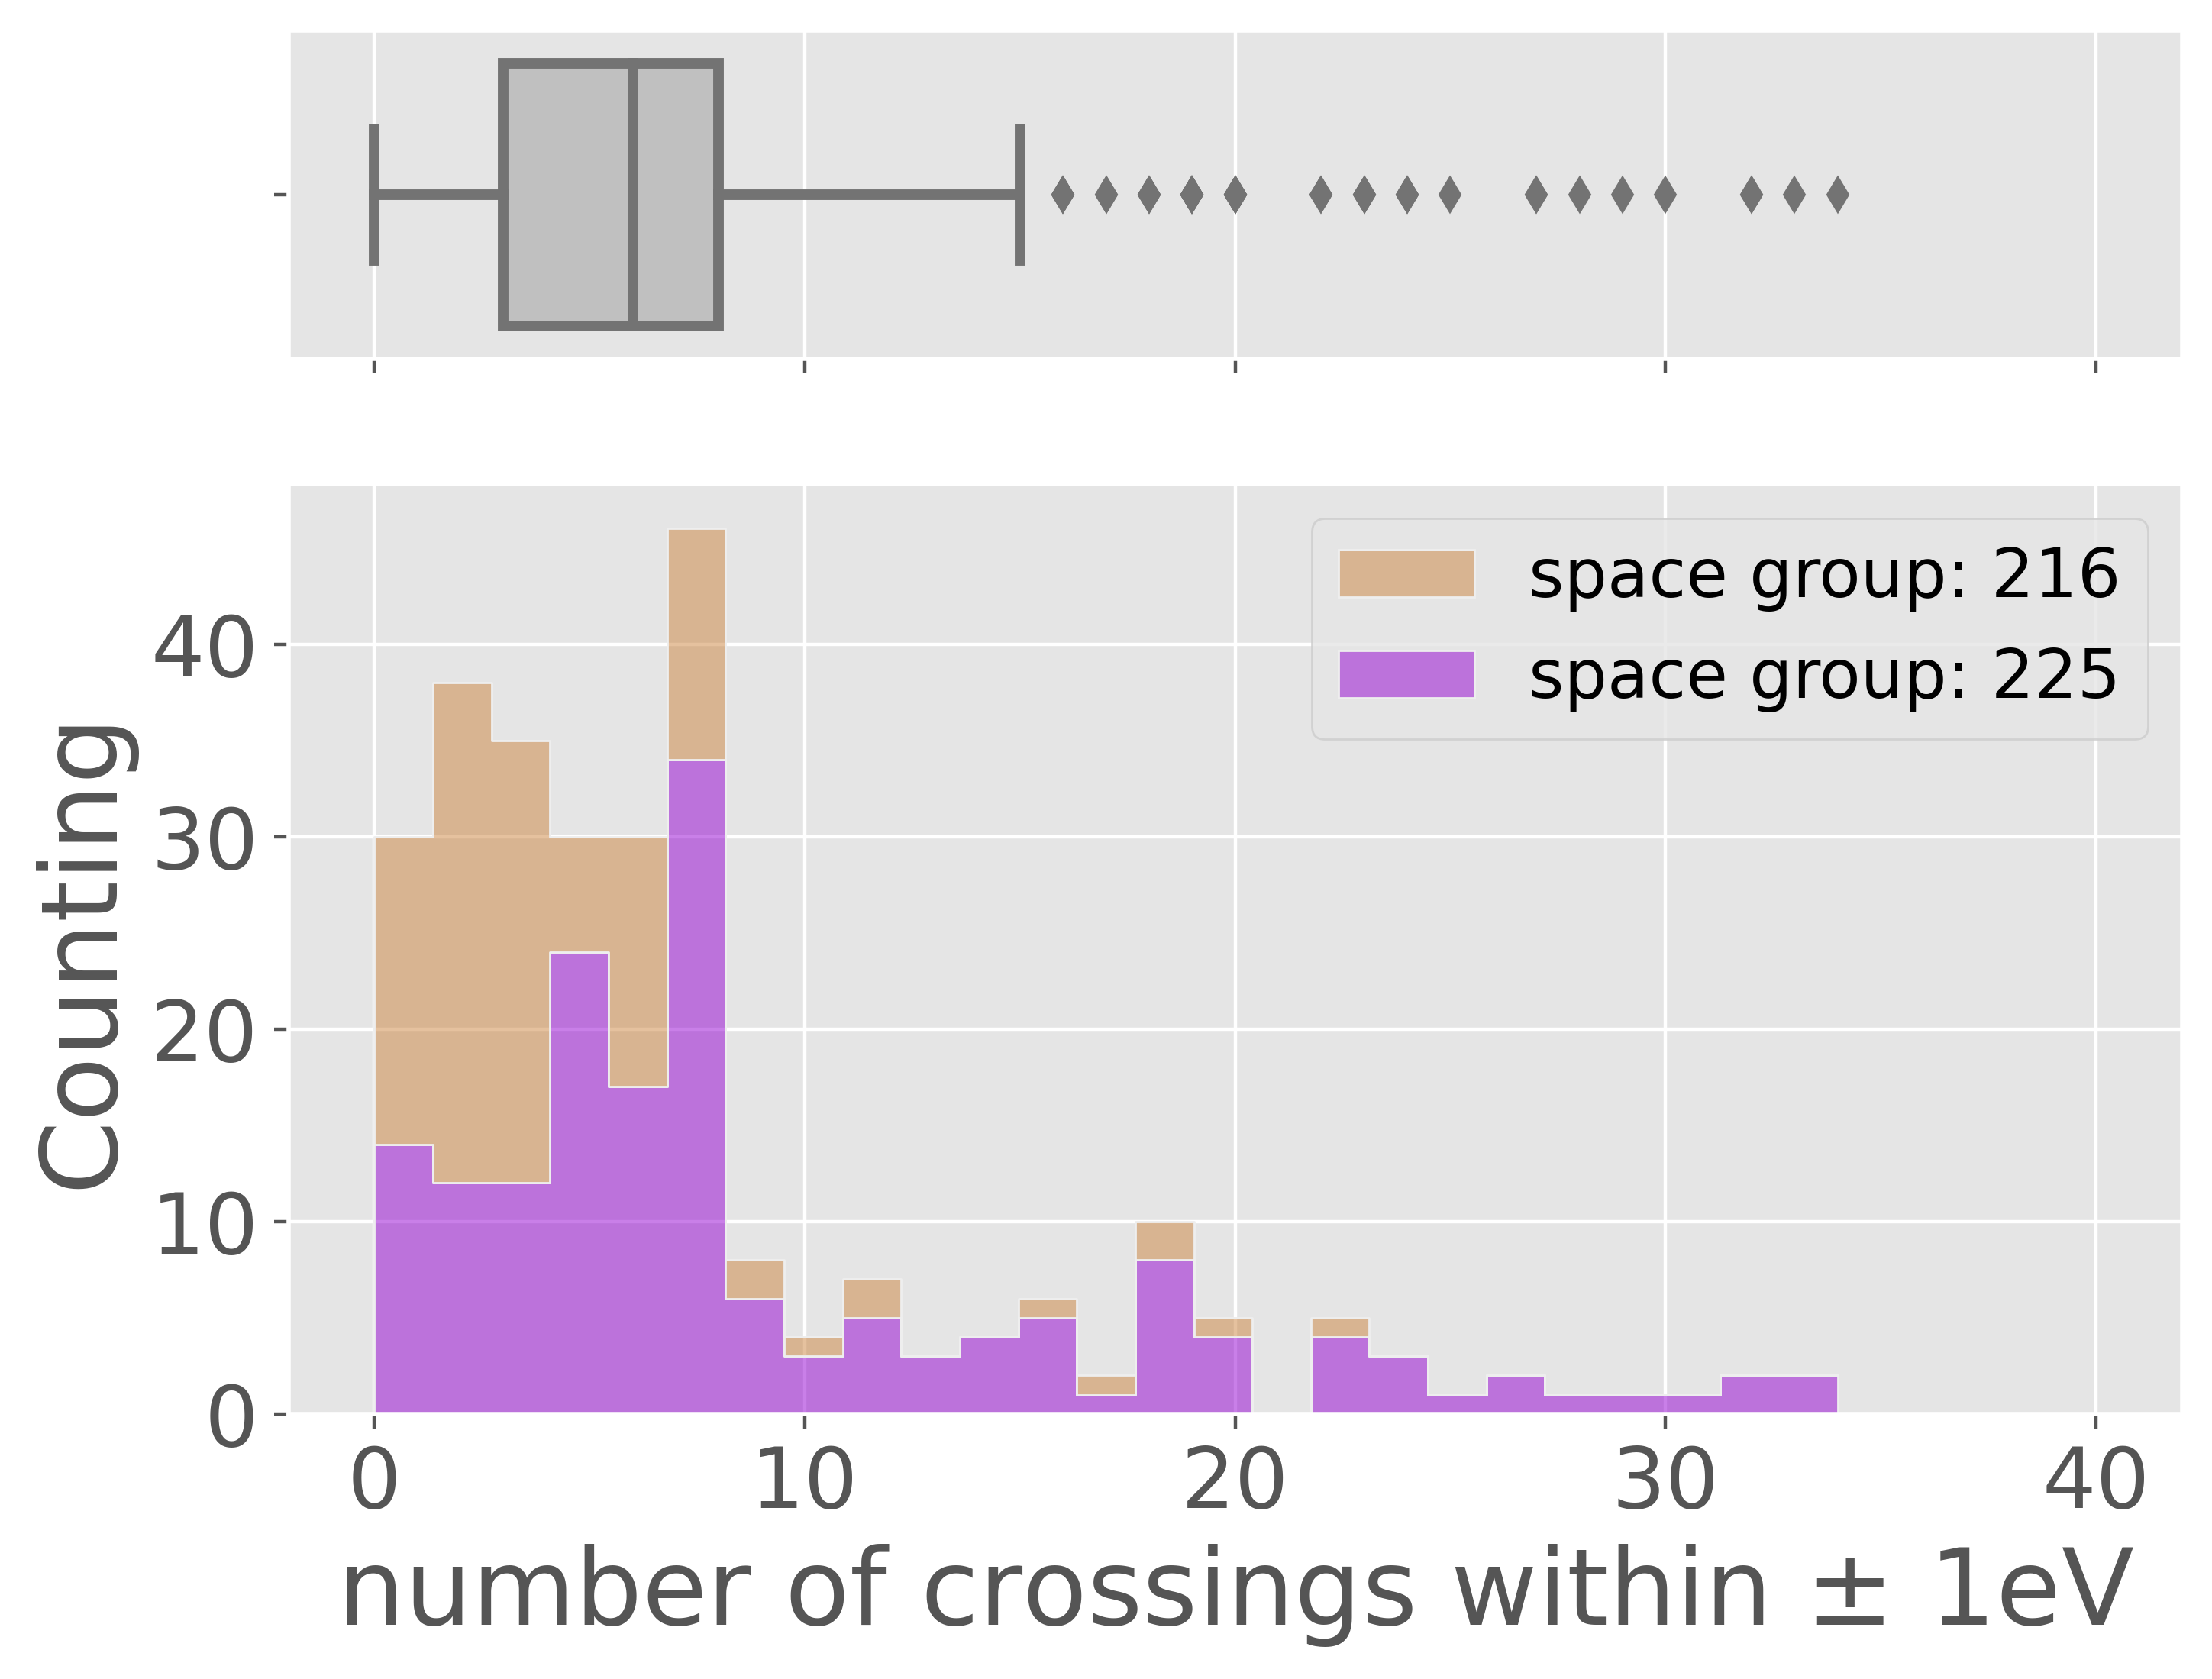
\includegraphics[scale=0.29]{Figures/Heuslers_EBS_dist.png}
        \label{fig:small_dataset_croos}
        }
        \quad
        \subfigure[]{
        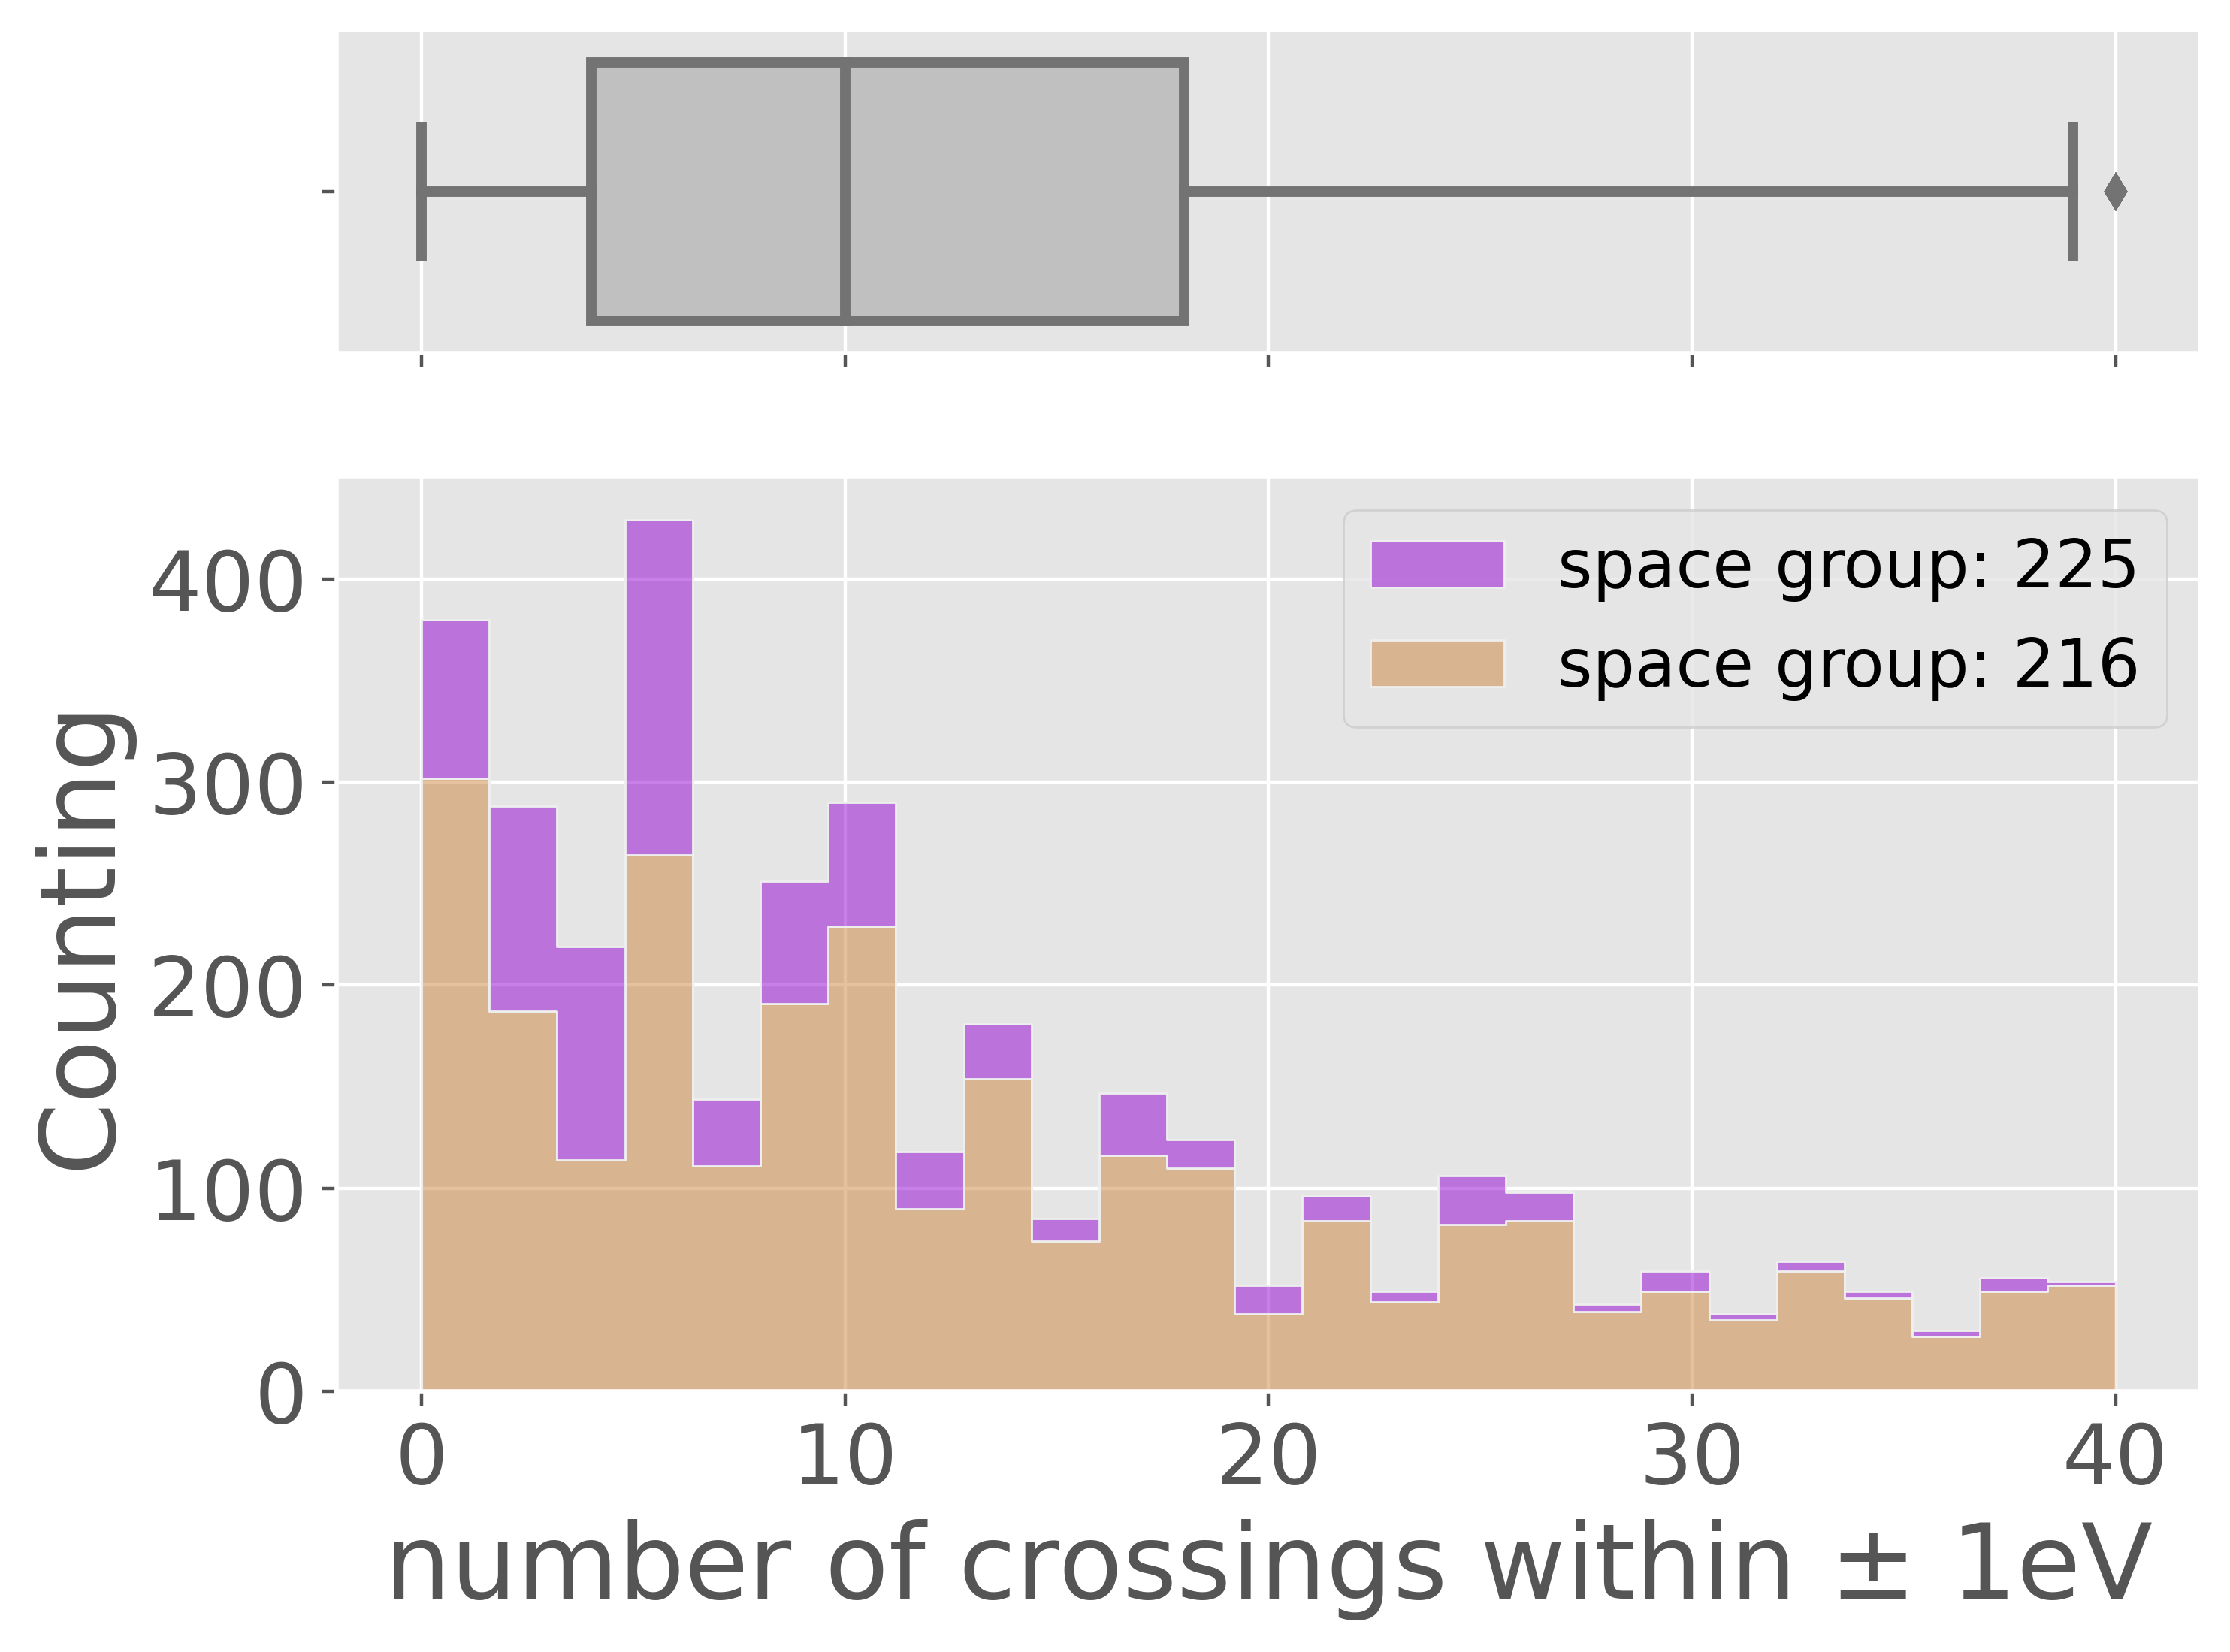
\includegraphics[scale=0.29]{Figures/Cubic_EBS_dist.png}
        \label{fig:big_dataset_croos}
        }
\caption{Distribution of number of crossings on the EBS (within $\pm$\SI{1}{\electronvolt}) a) Heuslers dataset, and b) Cubic dataset. [Colors online]}
\label{fig:dataset_croos}
\end{figure}
%\textcolor{pink}{Volha}
%Originally, we focused our attention on the materials with half-Heusler and full-Heusler compounds. Our  main objective was and stay to predict quantum features using one of machine learning approaches instead of the commonly utilized quantum mechanical calculation approach. In order to address this challenge, we decided to utilize XGBoost approach as an efficient and flexible technique for supervised learning (ref here: https://xgboost.readthedocs.io/en/stable/) 
%small dataset insists of 452 samples of materials which contains half-Heusler and full-Heusler compounds using our material search tool (ref. to Ale's description) with a few local properties: material mp id, chemical formula, lattice parameter, space group, and band structure. Further, we started our search of a set of relevant features that are powerful enough to capture the insight of our raw data.  During data mining and our search for a set of optimal local features, we generated and investigated features extracted based on structural properties, site properties, ionisation property, number of electrons, and chemical composition  of materials. Further, the materials with elements from f-block were eliminated. As a result, a dataset with 281 samples and 42 features was created. It is obvious that the created dataset is rather small. In the feature selection step we evaluated feature correlation and estimated their importance using XGBoost built-in feature importance module. Although, XGBoot approach is unaffected by multicollinearity, features with high correlation were eliminated. Further we focused on feature importance. Our experiments showed that approximately 10 of generated features had a very small or no impact on the prediction results and could be removed. We could not name the exact number because of BayesSearchCV function that we utilized for optimization of hyperparameter search. Finally, feature values were scaled. 
%My features:
%['lattice\_parameter',
% 'crossings\_+-1eV',
% 'density',
% 'vpa',
% 'packing fraction',
% 'max packing efficiency',
% 'ewald\_energy\_per\_atom',
% 'structural complexity per atom',
% 'frac s valence electrons',
% 'frac p valence electrons',
% 'frac d valence electrons',
% 'frac f valence electrons',
% 'avg ionic char',
% 'HOMO\_energy',
% 'LUMO\_energy',
% 'gap\_AO',
% 'range oxidation state',
% 'CovalentRadius\_0',
% 'CovalentRadius\_1',
% 'CovalentRadius\_2',
% 'FirstIonizationEnergy\_2',
% 'SecondIonizationEnergy\_2',
% 'ElectronAffinity\_2',
% 'Electronegativity\_2',
% 'AtomicRadius\_2',
% 'FirstIonizationEnergy\_1',
% 'SecondIonizationEnergy\_1',
% 'ElectronAffinity\_1',
% 'Electronegativity\_1',
% 'AllenElectronegativity\_1',
% 'AtomicRadius\_1',
% 'FirstIonizationEnergy\_0',
% 'SecondIonizationEnergy\_0',
% 'ElectronAffinity\_0',
% 'Electronegativity\_0',
% 'AllenElectronegativity\_0',
% 'AtomicRadius\_0',
% 'Ionisation\_0',
% 'Ionisation\_1',
% 'Ionisation\_2',
% 'Electrons\_0',
% 'Electrons\_1',
% 'Electrons\_2']

\subsection{Machine Learning Modeling}
\begin{figure}[H]
    \centering
    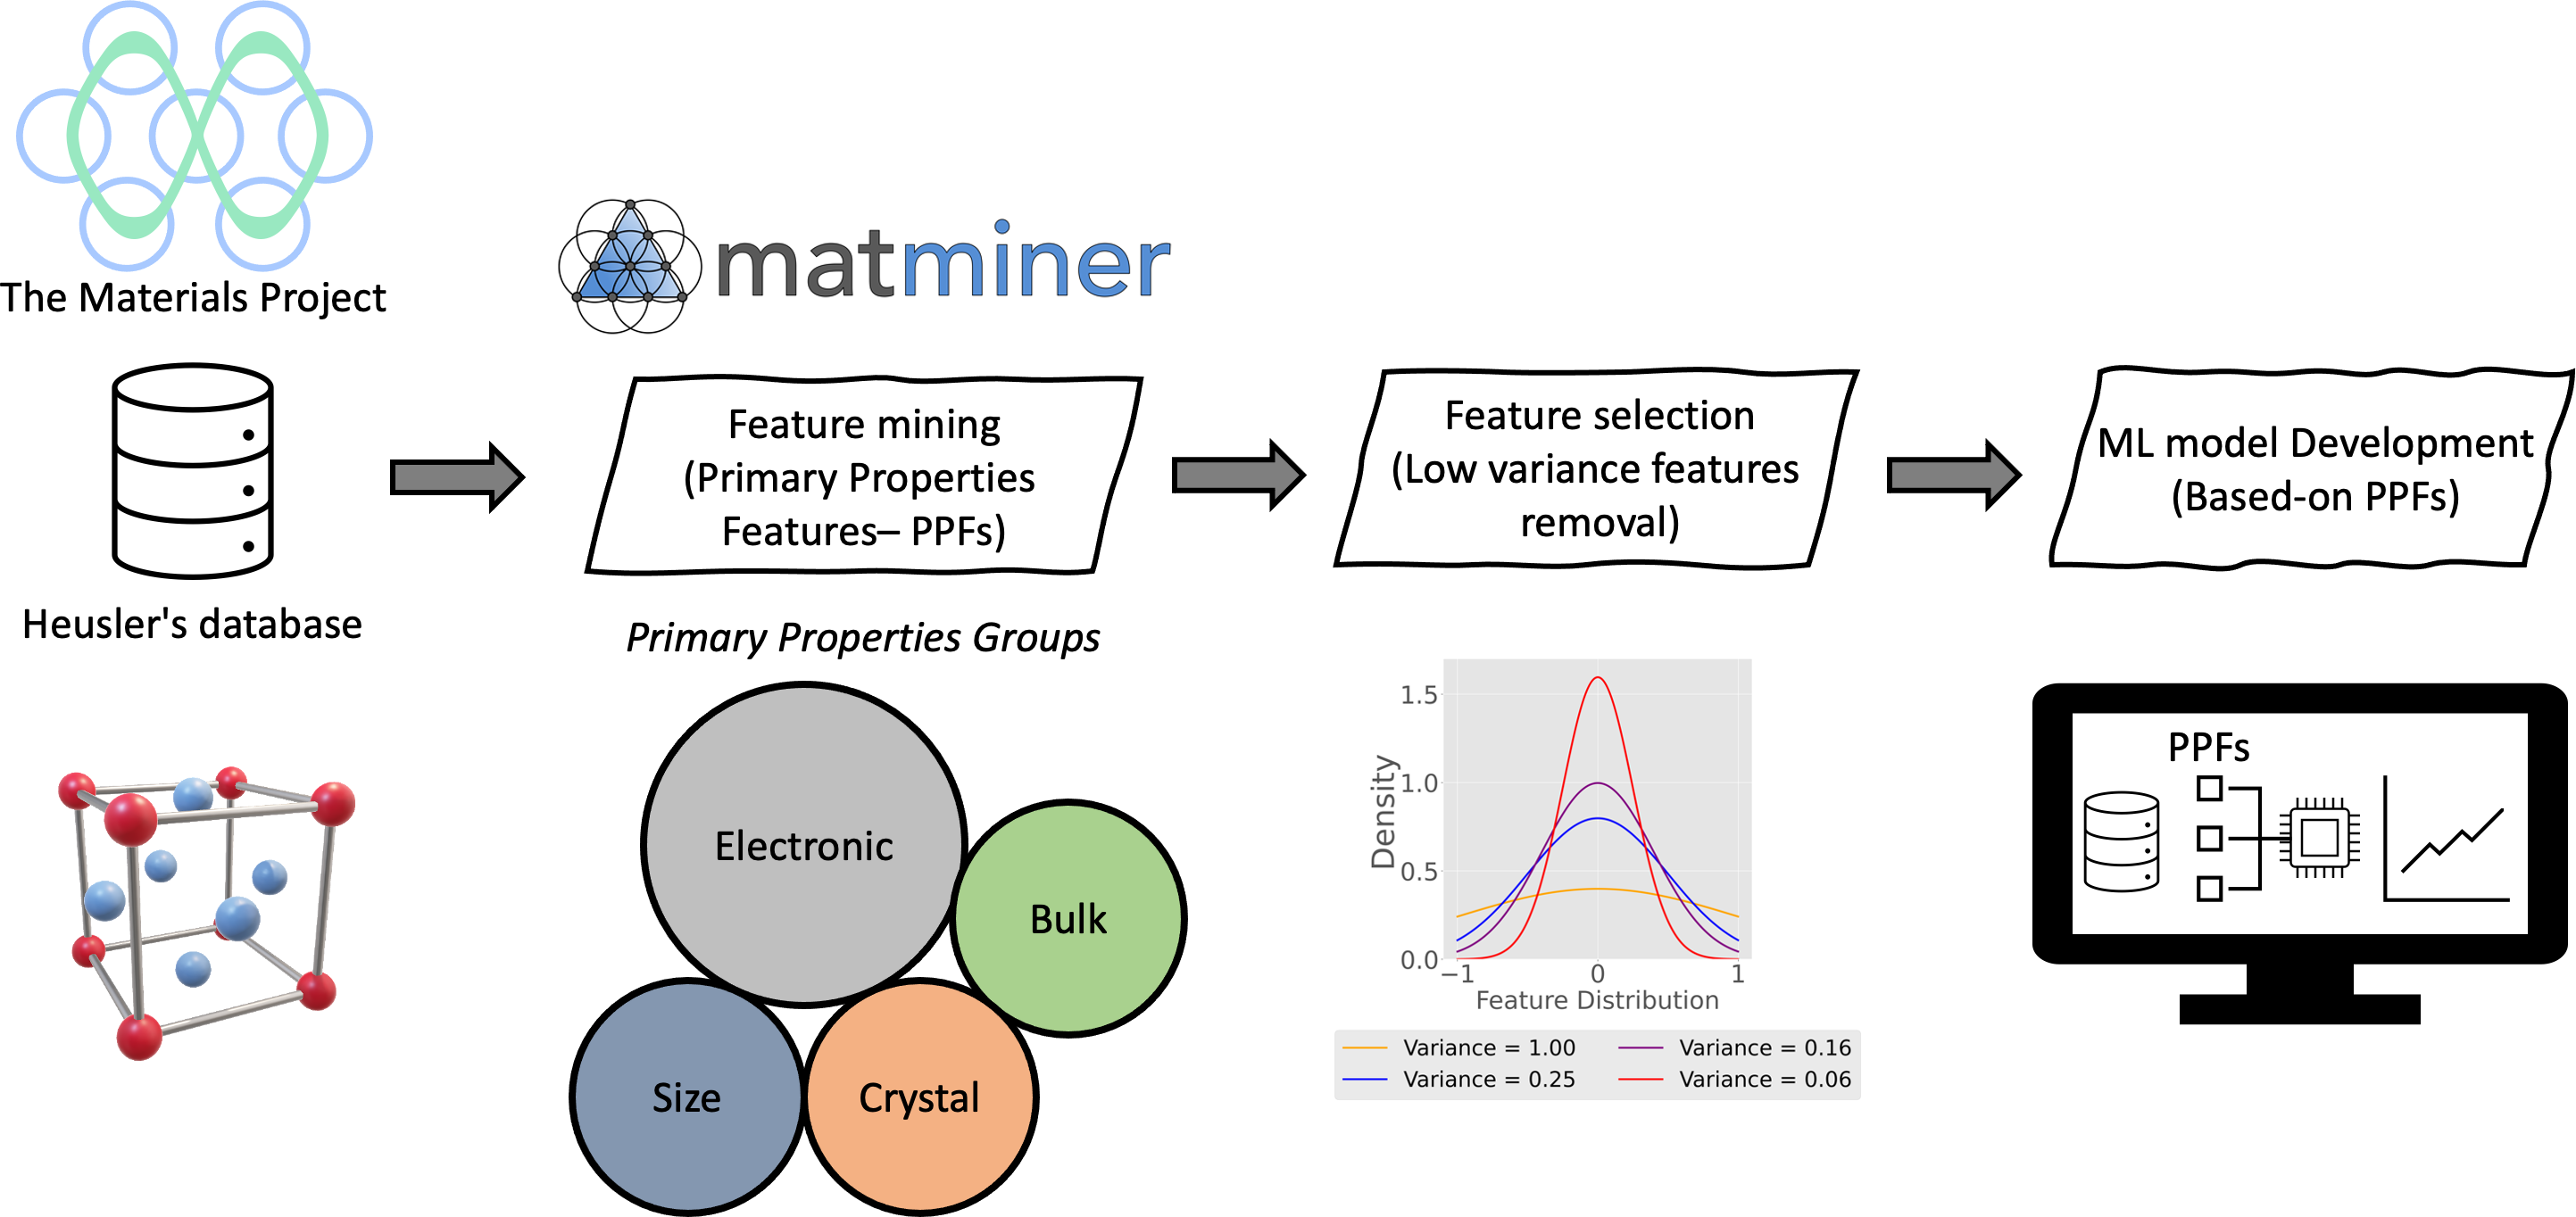
\includegraphics[width=0.7\textwidth]{Figures/FeatureEngineeringSkin.png}
    \caption{ML modeling flowchart; which consist of: 1) data minig and data sets creation, 2) features extraction, 3) features selection, and 4) ML models development. [Colors online]}
    \label{fig:MLWorkFlow}
\end{figure}

A Machine learning (ML) pipeline is implemented to develop models that can predict the number of crossings in the EBSs (within $\pm$\SI{1}{\electronvolt}) for the Heuslers and Cubic datasets. From the logic that the EBS's number of crossings depends on the nature of the atoms within the crystal lattice and their arrangement with each other, the models take as the input as the identities of the atoms in the crystal---encoded as elemental properties---producing, as output, estimates of the number of crossings (within $\pm$ \SI{1}{\electronvolt}). A general flowchart for ML pipeline is presented on Figure \ref{fig:MLWorkFlow}; specifically, the features engineering consists of two main steps: 1) Feature extraction, and 2) Feature selection. For features extraction, atom properties are taken from the python library Matminer\cite{ward2018matminer,Matminer} for both datasets and named primary properties features (PPFs) and are classified into 4 groups: bulk, electronic, size, and crystal. Matminer creates overall features i.e., for a specify elemental composition of a crystal, and identifies the minimum and maximum values for a given property. We consider a total of 53 PPFs including e.g, electronegativity, covalent radius, volume per atom, etc.  %\textcolor{red}{To improve ML models prediction performances, our feature engineering skin also incorporate the construction of suitable descriptors from the given PF. This feature engineering skin involves the application of a transformation function, i.e. the multiplication of minimum and maximum values for a given PF for generating new descriptor named combined feature (CF).} 
The PPFs, for developing the ML models, are selected based on the low-variance criterion; i.e. any given PPF which consists of a constant value in the \SI{80}{\percent} or more of its values distribution, or whose variance is $\mathrm{\leq}$ \num{0.16}, are removed. See SI for the full list of PPFs and their values. %\textcolor{red}{Importantly, these PPFs consider?}  %Several tree-based ML algorithms, such as Random forests and Gradient Boosting, can be good at detecting interactions between different features, but highly correlated features can mask these interactions. For that reason  lowly correlated features are prefered to be used for training ML models. Since more than \textcolor{red}{\SI{70}{\percent}} of the regressors are highly correlated (see Figure \ref{fig:PFCorrelation}), highlighting the low correlation between PFs and CFs; we implement a feature extraction skin based-on principal component analysis (PCA). Thus generating a set of uncorrelated principal component features herein named PCFs (see Figure \ref{fig:PCFCorrelation}); moreover, how the PCFs are related to PFs and CFs is depicted on Figure \ref{fig:eigenvectors} by using a heatmap representation. The final number of selected PCFs are based on the variance explained by each of the PCFs (\textcolor{red}{see Figure S.tal}).

%\begin{figure}[H]
%        \subfigure[]{
%        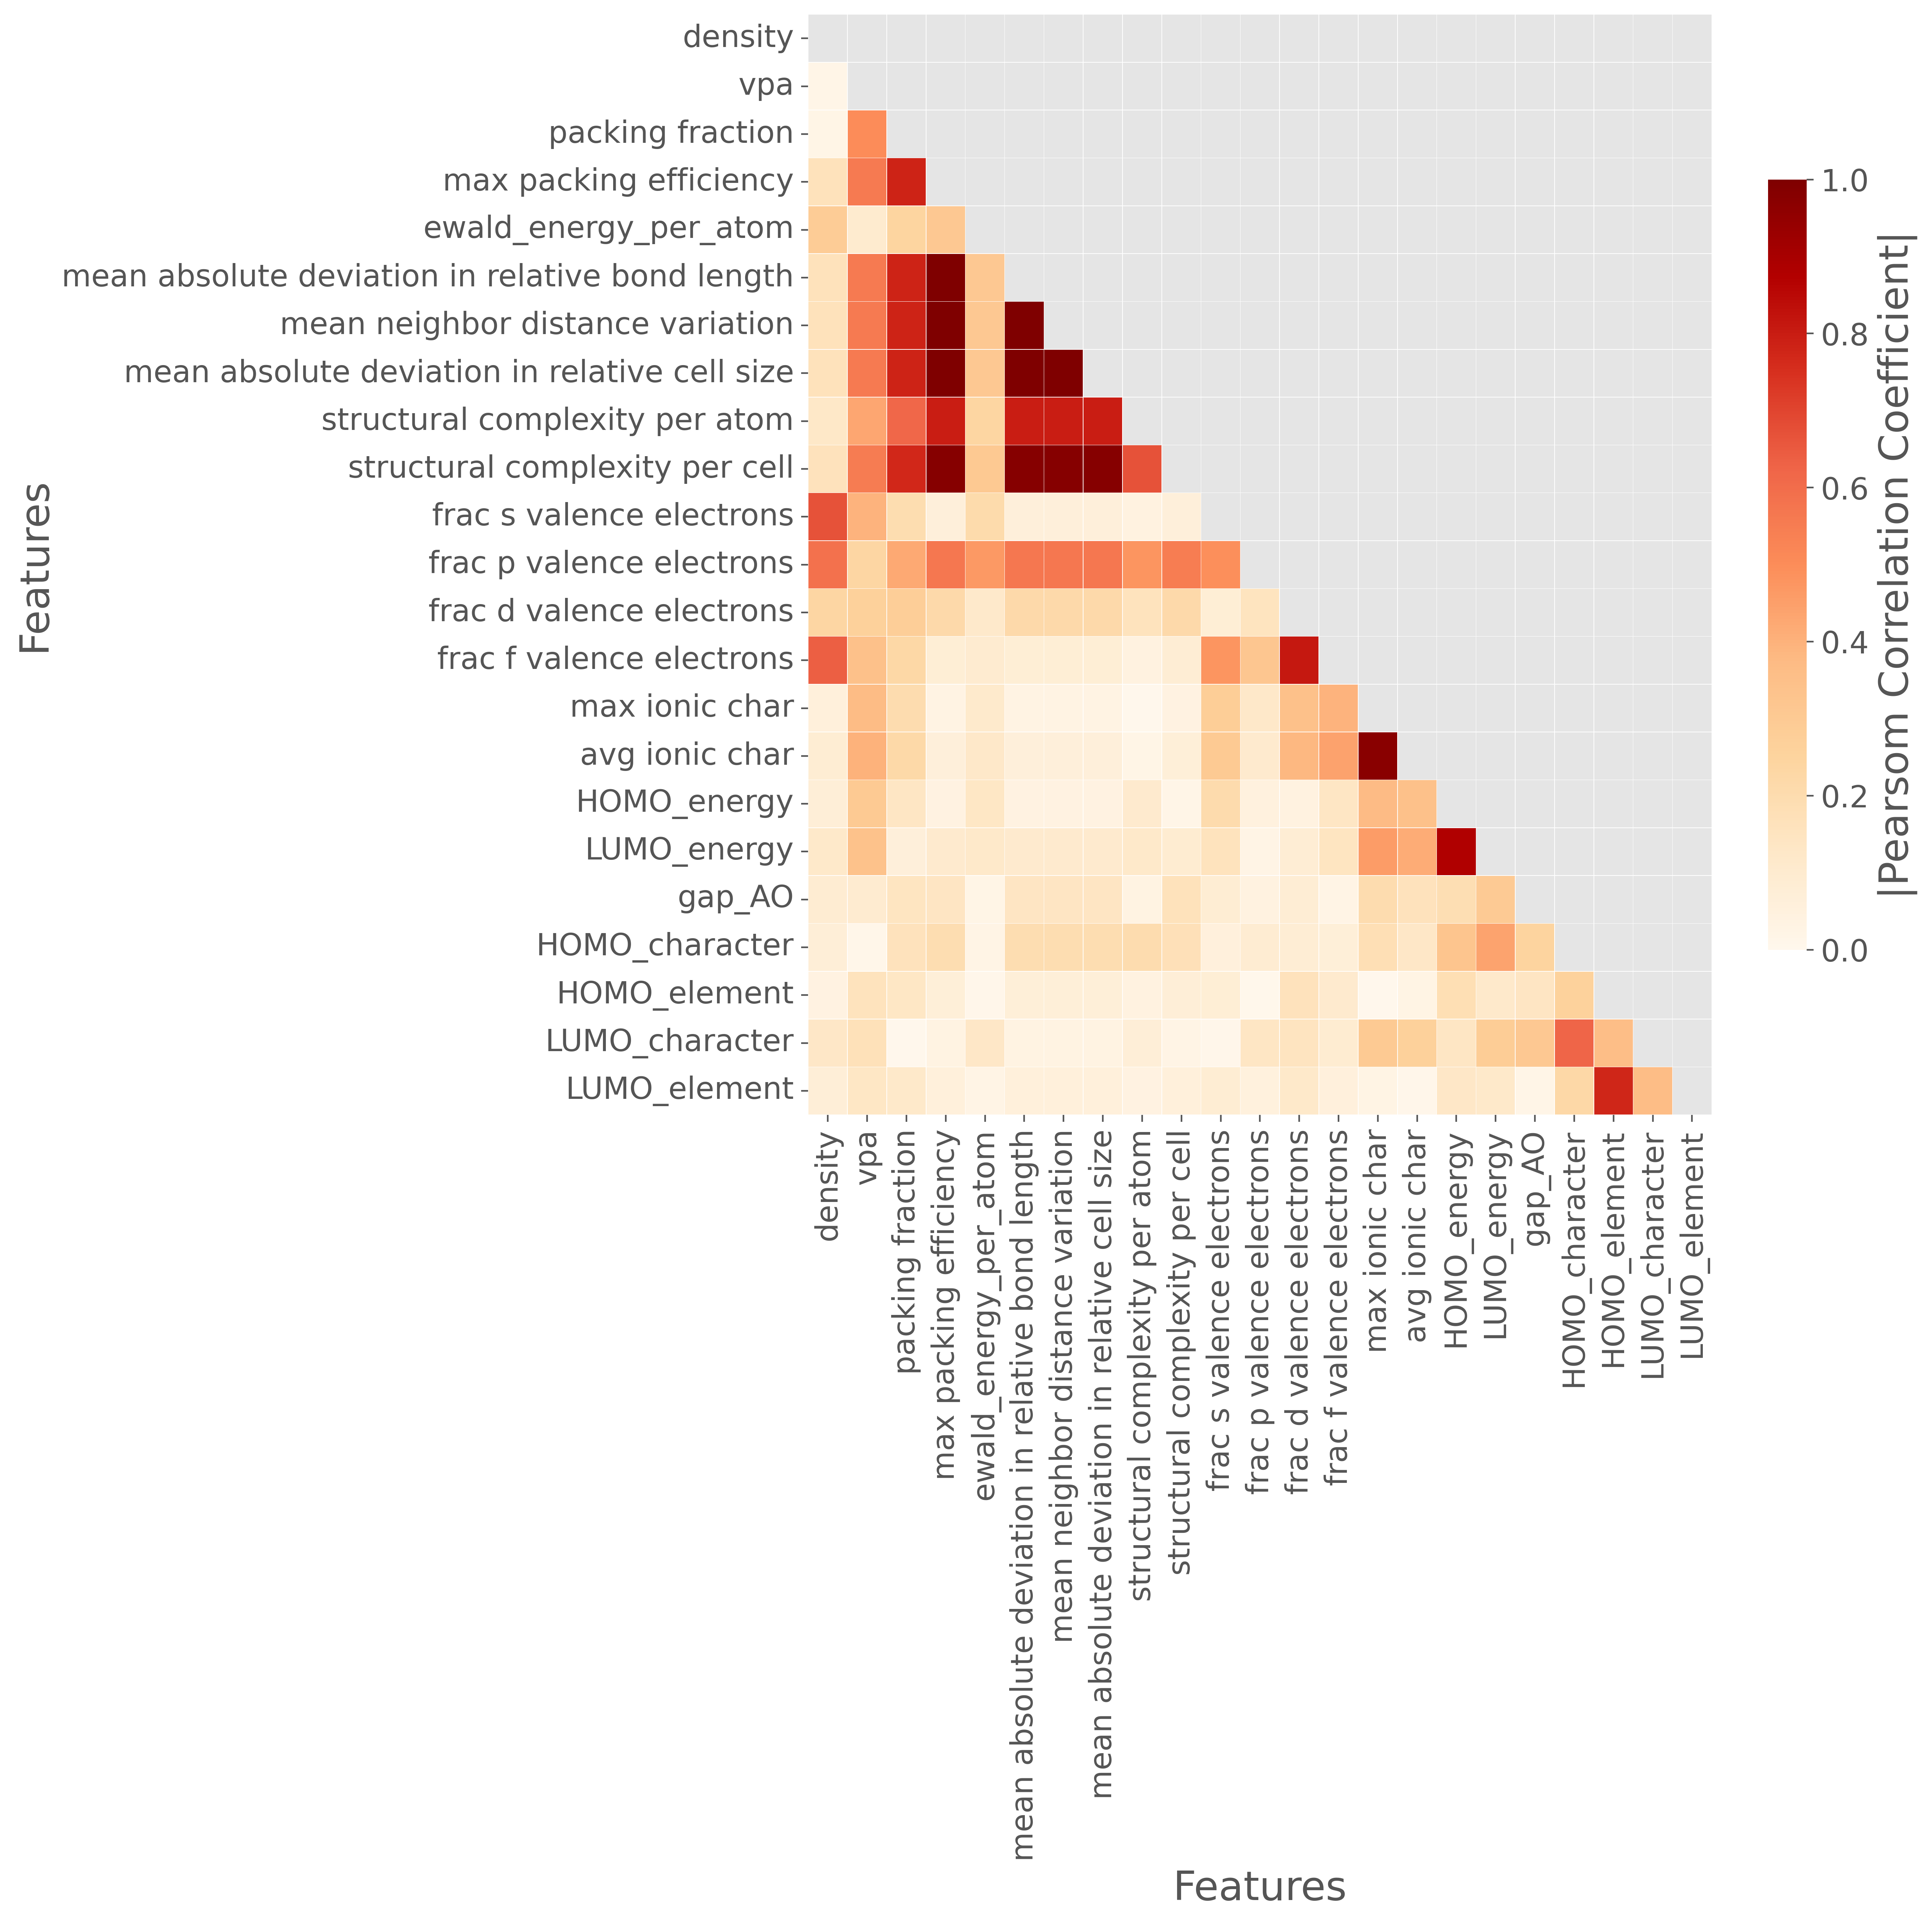
\includegraphics[width=3.0in]{Figures/Heusler_Feature_Correlation_Pearson.png}
%        \label{fig:small_dataset_croos}
%        }
%        \quad
%        \subfigure[]{
%        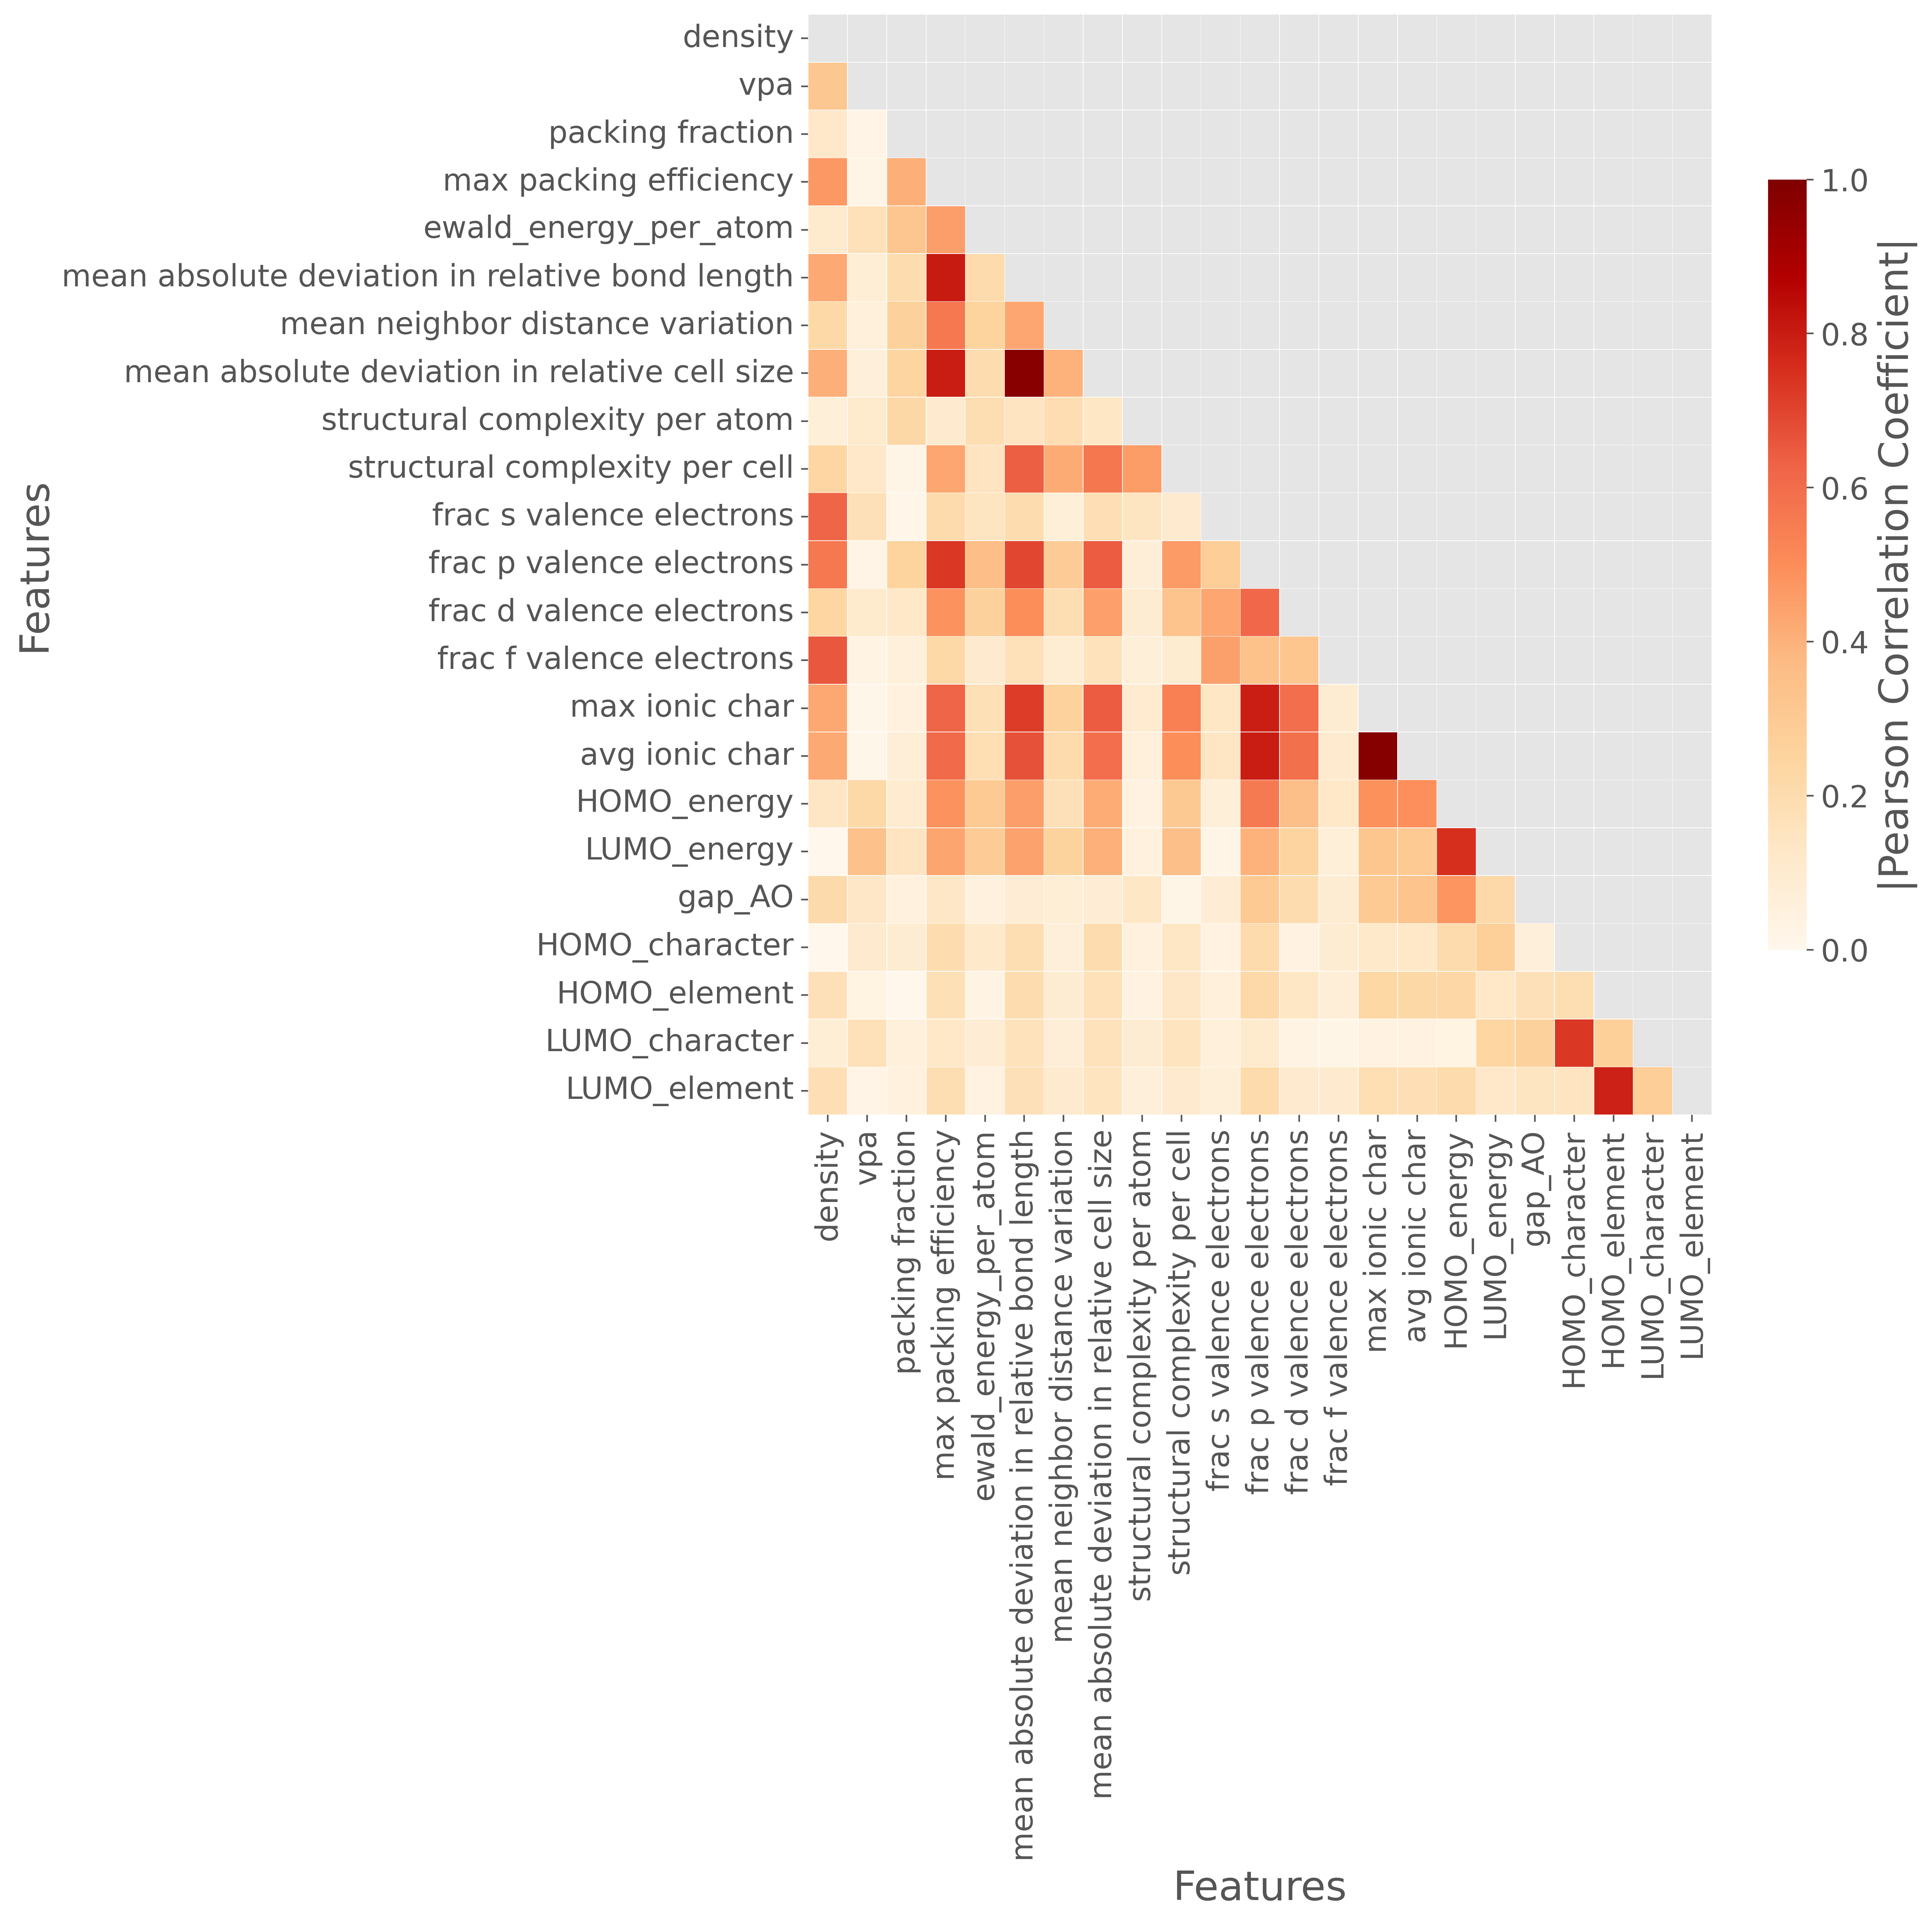
\includegraphics[width=3.0in]{Figures/Cubic_Feature_Correlation_Pearson.png}
%        \label{fig:big_dataset_croos}
%        }
%\caption{PPFs Pearson correlation coefficient absolute value ($|\mathrm{r}|$) heatmaps for a) Heusler and b) Cubic datasets compounds. The color scale represents gradient for non-correlated features ($|\mathrm{r}| = 0.0$ -- white) and strong correlated features ($|\mathrm{r}| = 1.0$ -- red). [Colors online]}
%\label{fig:PFCorrelation}
%\end{figure}

%\begin{figure}[H]
%\centering
%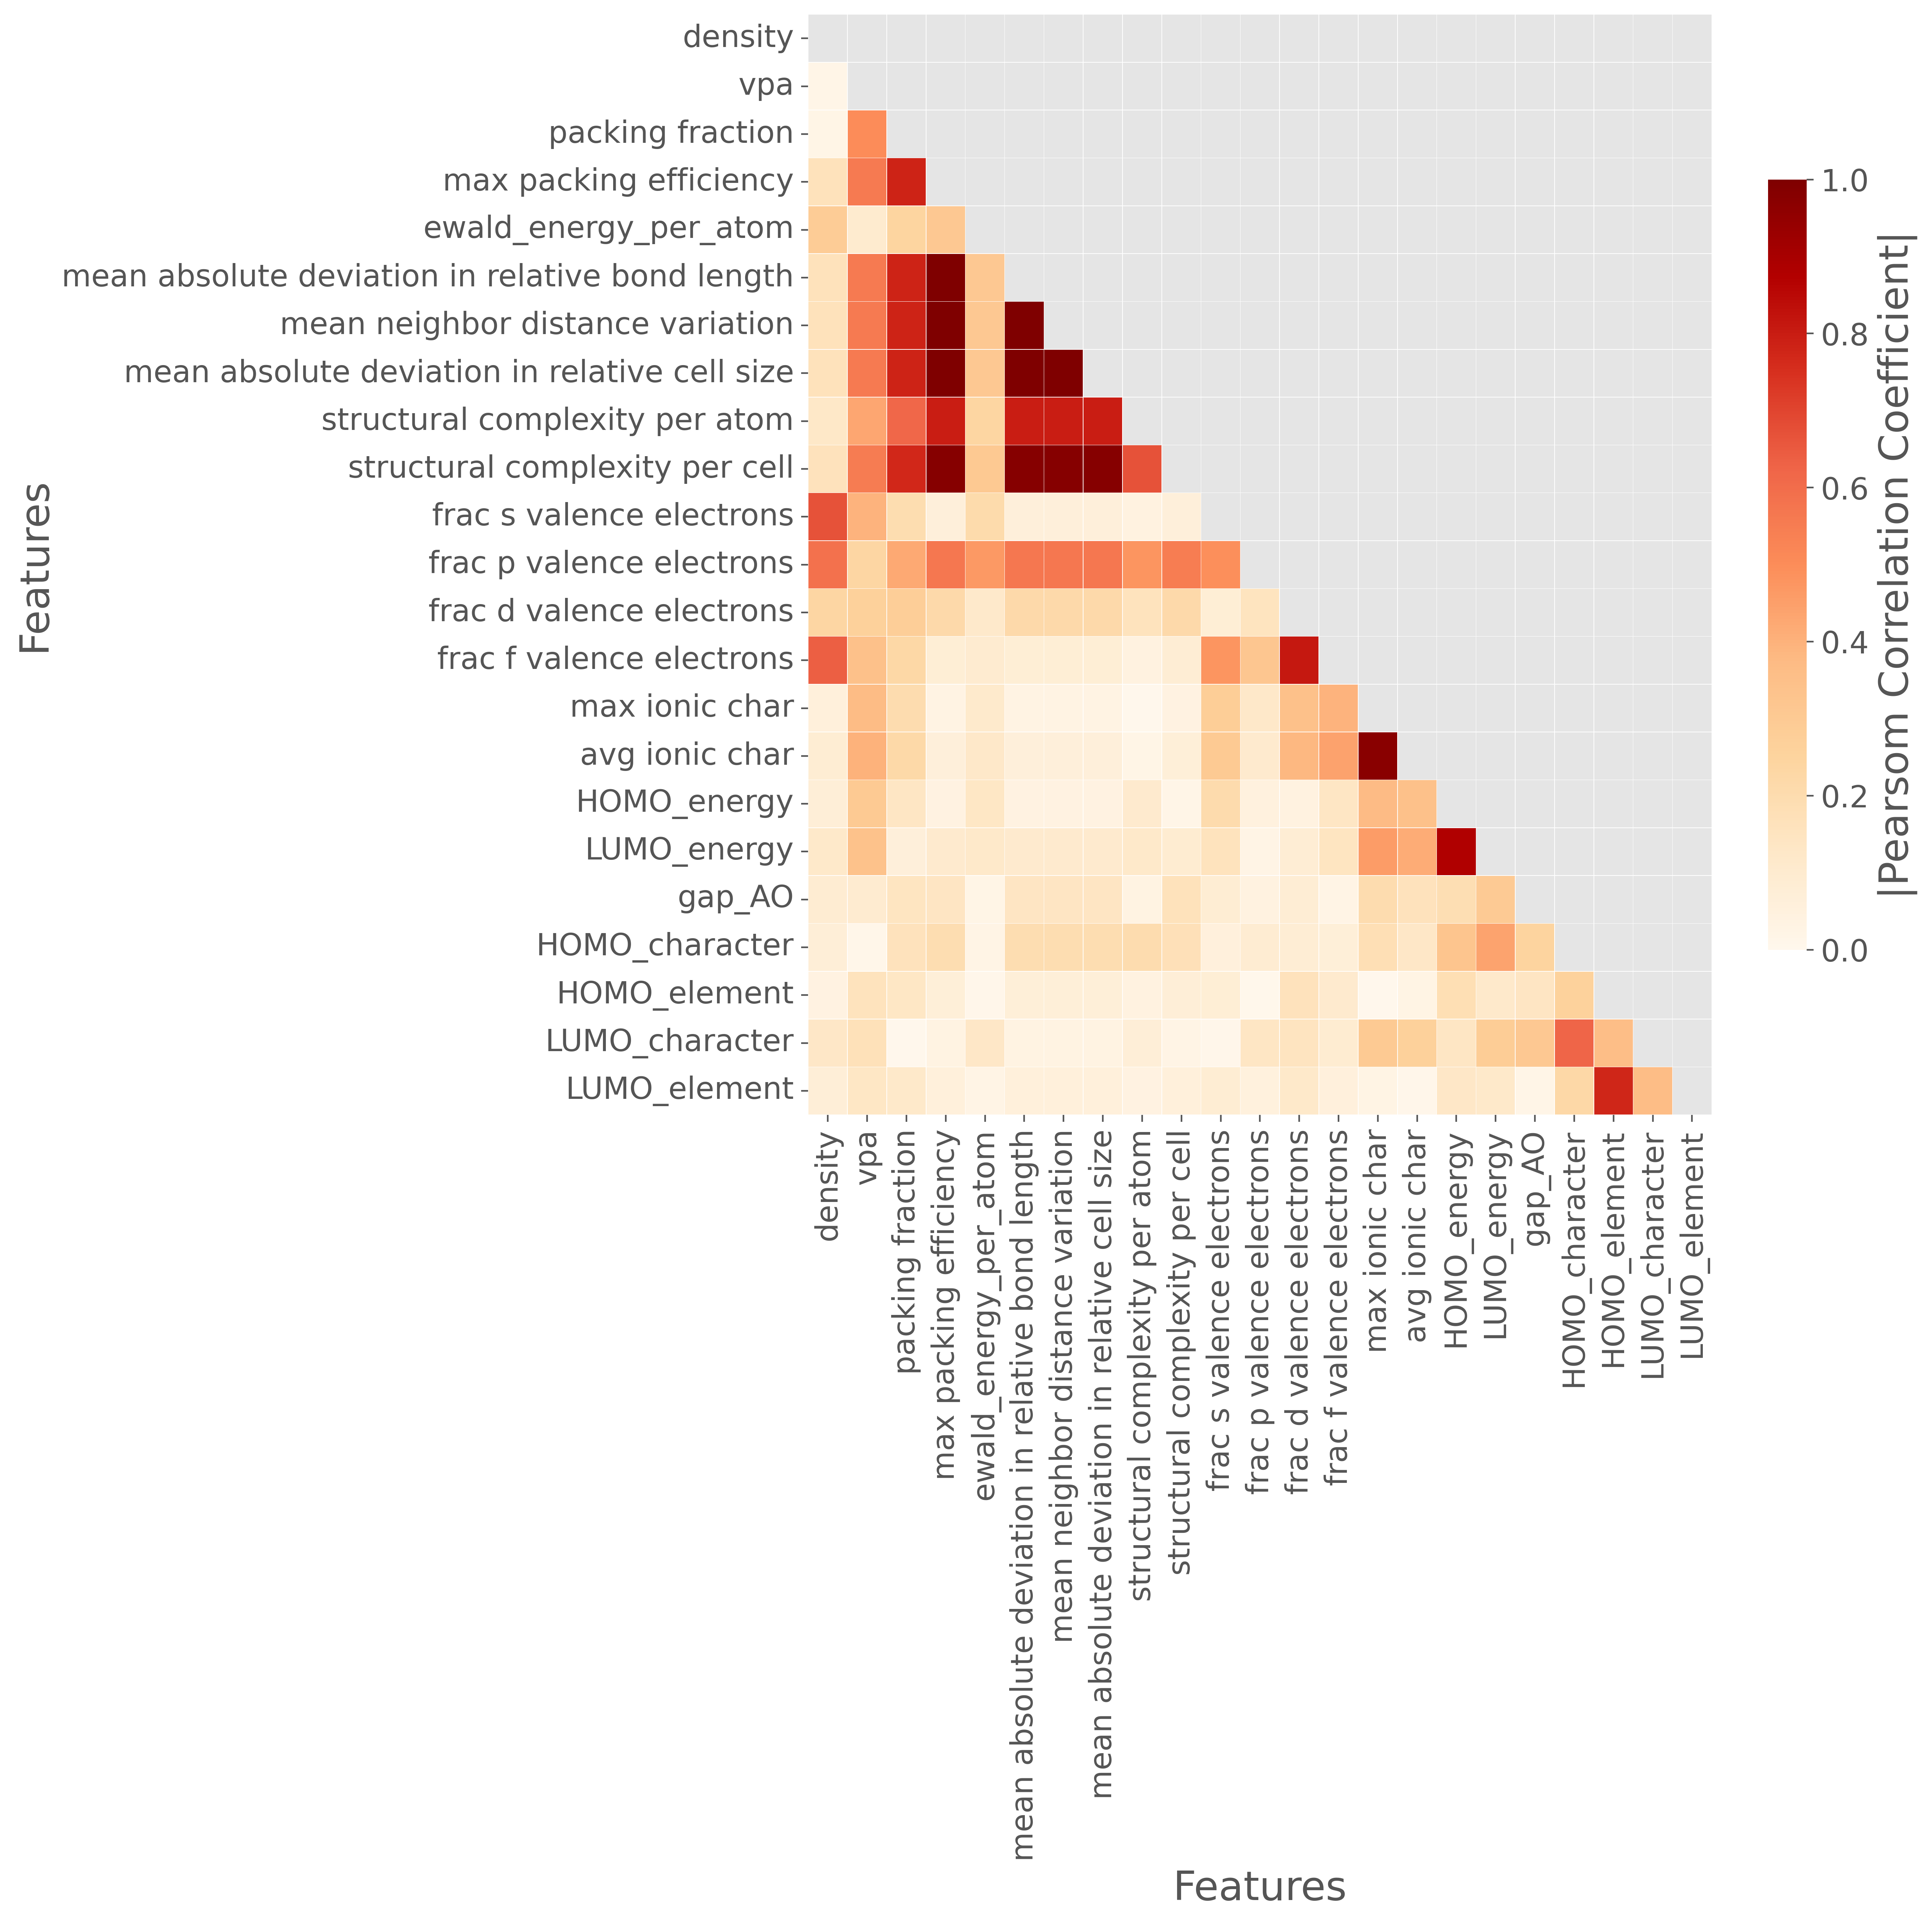
\includegraphics[scale=0.25]{Figures/Heusler_Feature_Correlation_Pearson.png} 
%\caption{PPFs Pearson correlation coefficient absolute value ($|\mathrm{r}|$) heatmap. The color scale represents gradient for non-correlated features ($|\mathrm{r}| = 0.0$ -- white) and red represents strong correlated features ($|\mathrm{r}| = 1.0$ -- white). [Colors online]}
%\label{fig:PFCorrelation}
%\end{figure}

%\begin{figure}[H]
%\centering
%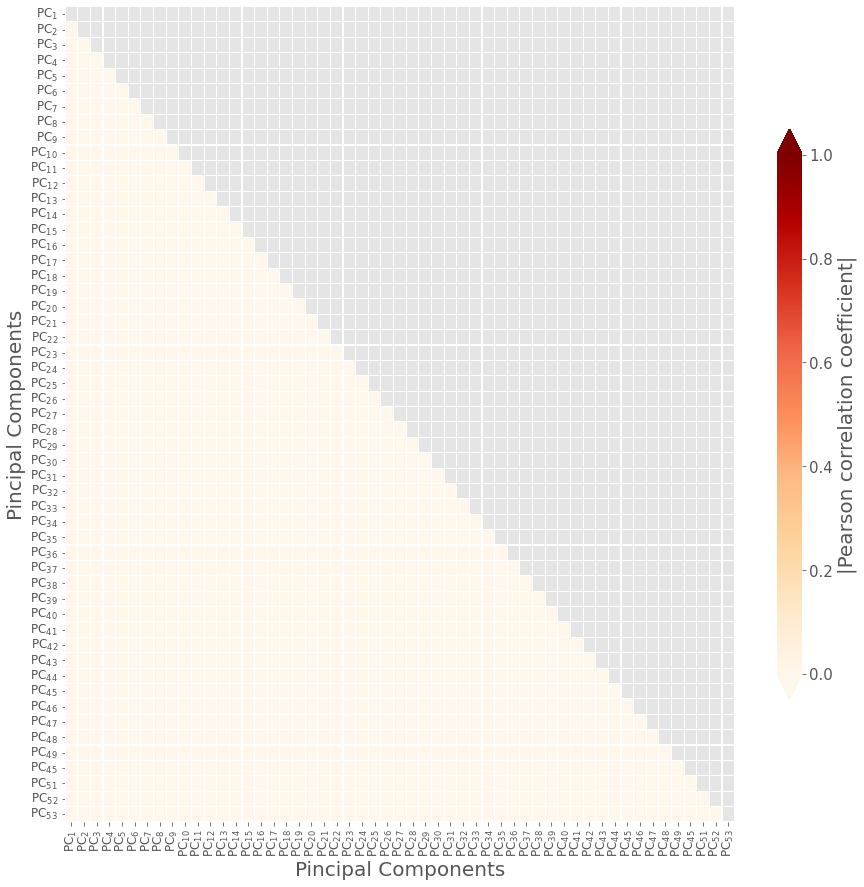
\includegraphics[scale=0.30]{Figures/PCF-Correlation_HM.png} 
%\caption{Pearson correlation coefficient. [Colors online]}
%\label{fig:PCFCorrelation}
%\end{figure}

%\begin{figure}[H]
%\centering
%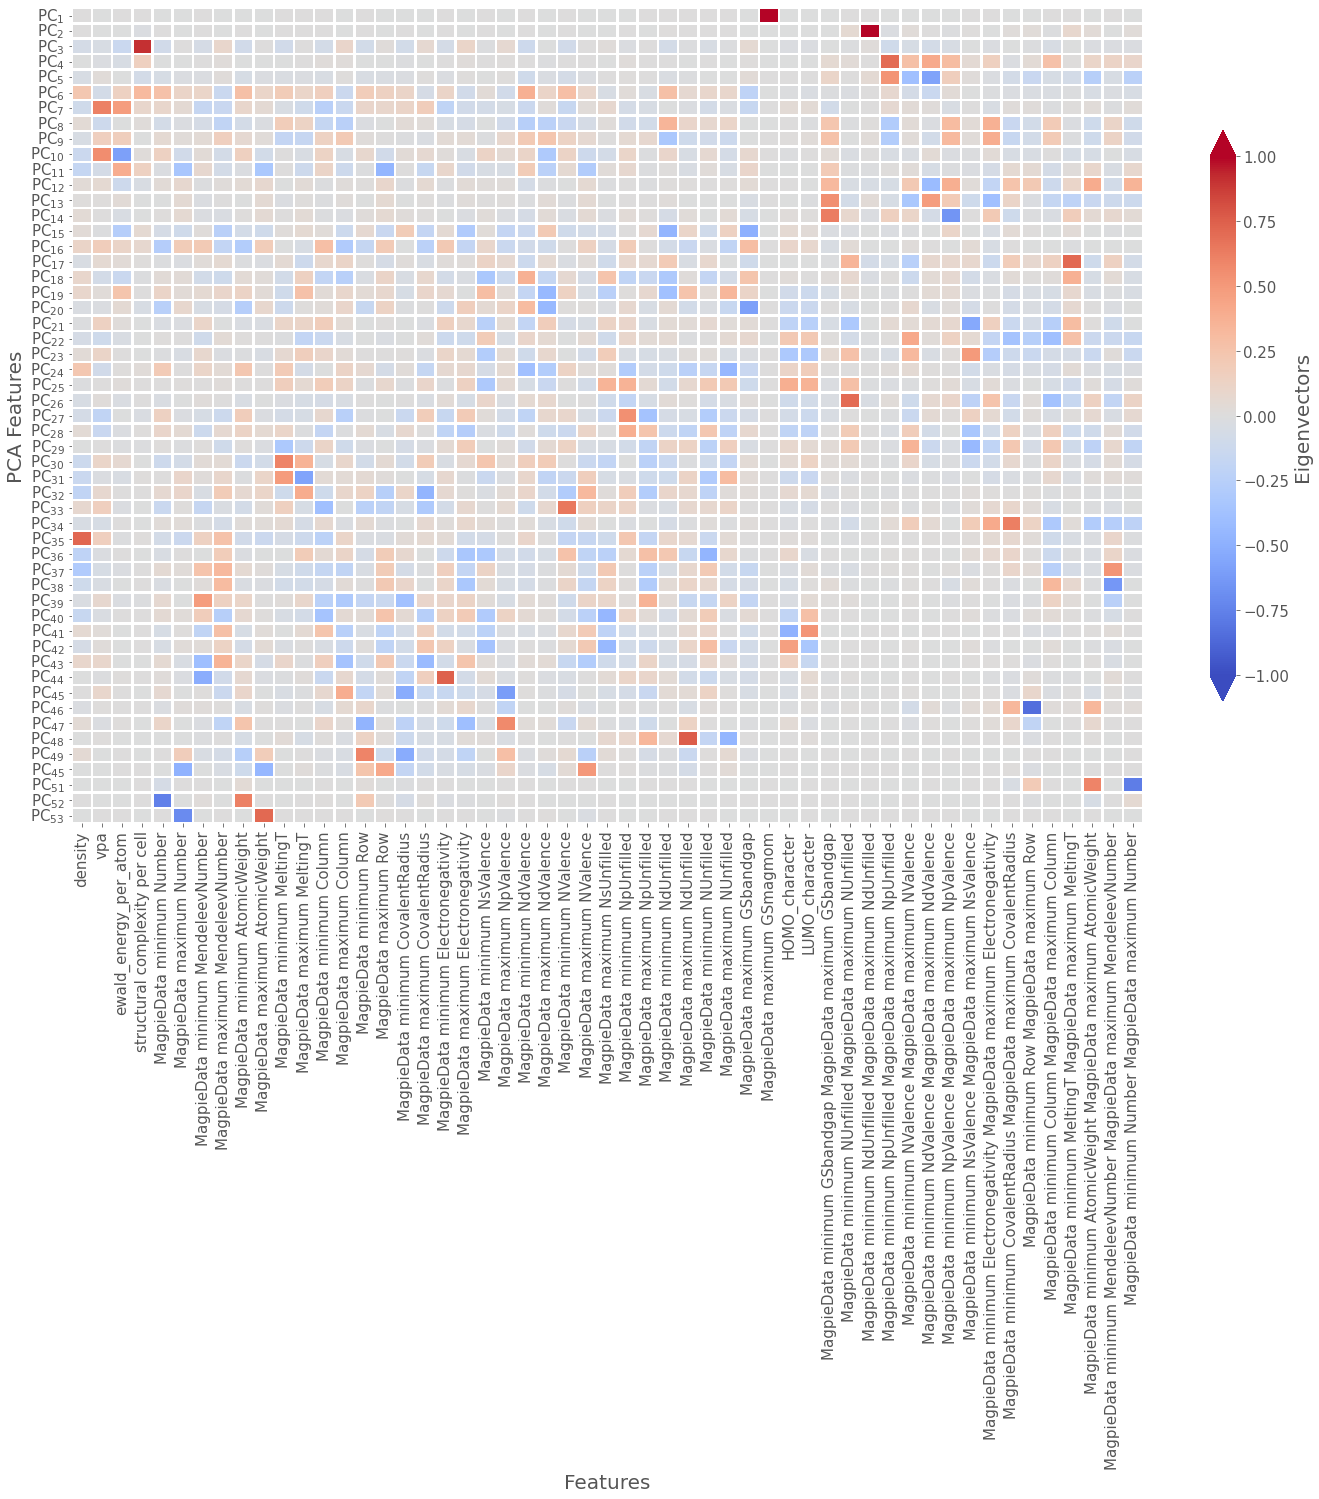
\includegraphics[scale=0.30]{Figures/PCA_eigenvectors.png.png} 
%\caption{Pearson correlation coefficient. [Colors online]}
%\label{fig:eigenvectors}
%\end{figure}

The ML regression models and features importance are performed with the XGBoost approach \cite{chen2015xgboost,chen2016xgboost}. XGBoost provides a parallel tree boosting algorithm \cite{chen2008trada} that contains three elements: 1) a minimizing loss function, 2) a weak learner (regression tree) for making predictions, and 3) an additive model that combines weak learners into strong ones in order to minimize the loss function. In our model, the loss function is the root mean square error (rmse) between the computed and the ML predicted band structure number of crossings (within $\pm$\SI{1}{\electronvolt}). The regression trees weak learners are set by specifying the learning rate, gamma, max\_depth, max\_delta\_step, subsample, colsample\_bytree, colsample\_bylevel, lambda, alpha, gamma, min\_child\_weight, and scale\_pos\_weight parameters. Bayesian optimization and cross validation (shuffle-split (7-folded)) algorithms, as implemented in scikit-optimize python library,\cite{head_tim_2020_4014775} are employed to identify the best combinations of hyperparameter values (e.g., max depth, number of threads, etc.) during the ML-models development. The Feature importance score (using gain scoring) is estimated to identify those PPFs that most influence the prediction of band structure number of crossings (within $\pm$\SI{1}{\electronvolt}). %The features sensitivity is then assess, by analyzing the $\mathrm{R^2}$ of ML-model which recursively incorporate PPFs one at the time, protecting our reduced featured model against overfitting. 
%To asses the model validation, we implement the K-Fold cross-validation method\cite{ojala2010permutation} in 10 separate runs, in each one, the data is split randomly into ``test'' and ``training'' sets. 
\SI{70}{\percent} of the dataset is assigned to the training set, whereas the remaining \SI{30}{\percent} is assigned to the testing set. The training and test sets are assessed based on the mean absolute errors (MAEs) between the calculated (with DFT) and the predicted (with ML) as illustrated in eq. \ref{eq:MAE}:

\begin{equation} \label{eq:MAE}
\mathrm{
MAE = \frac{\sum_i^N \left|n_i^{DFT} - n_i^{ML}\right|}{N}
}
\end{equation}

\noindent where $\mathrm{n}$ stands for band structure number of crossing (within $\pm$\SI{1}{\electronvolt}).

\section{Results}
\subsection{Machine Learning Model}
\begin{figure}[H]
    \centering
        \subfigure[]
        {
        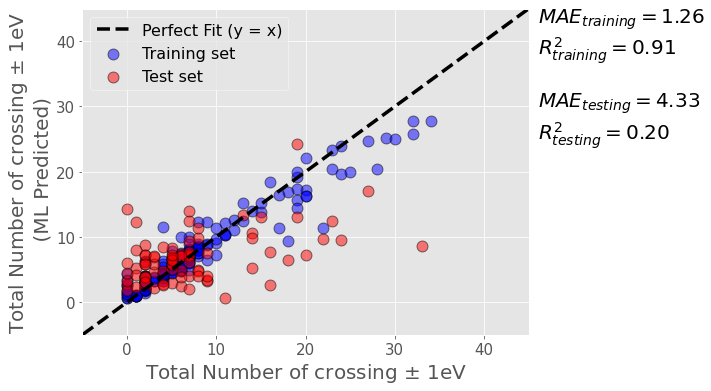
\includegraphics[width=3in]{Figures/Heuslers_ML-parity.png}  
        \label{fig:MLmodela}
        }
        \quad
        %\subfigure[]
        %{
        %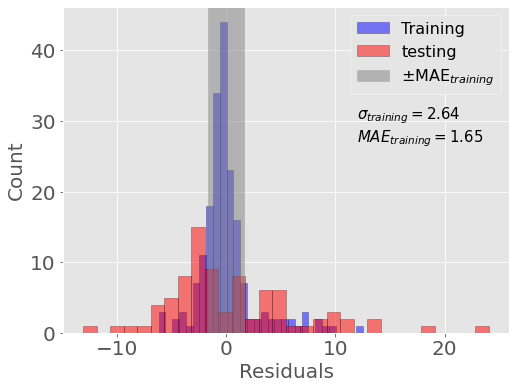
\includegraphics[scale=0.29]{Figures/Heuslers_residuals_dist.png}
        %\label{fig:MLmodelb}
        %}
        %\quad
        
        \subfigure[]{
        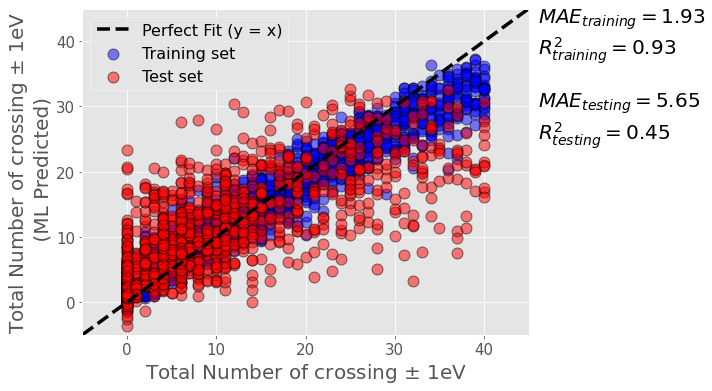
\includegraphics[width=3in]{Figures/Cubic_ML-parity.png}
        \label{fig:MLmodelb}
        }
        %\subfigure[]{
        %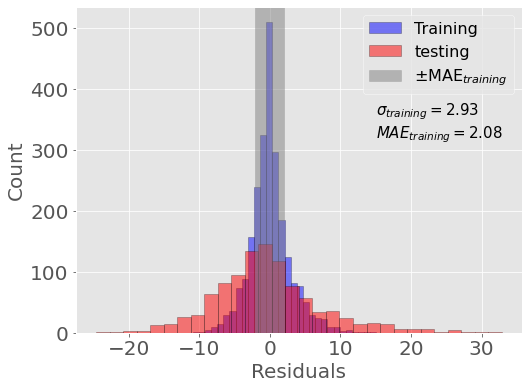
\includegraphics[scale=0.29]{Figures/Cubic_residuals_dist.png}
        %\label{fig:MLmodeld}
        %}        
\caption{ML model parity plot comparing DFT-calculated with ML predicted values for band structure number of crossing (within $\pm$\SI{1}{\electronvolt}) a) Heuslers dataset, and b) Cubic dataset. [Colors online]}
\label{fig:MLmodel}
\end{figure}

Figures \ref{fig:MLmodela} and \ref{fig:MLmodelb} compare, in parity plots, the ML predictions with DFT-calculated EBS's number of crossings (within $\pm$\SI{1}{\electronvolt}) for the Heuslers and Cubic datasets respectively. For these models, the coefficient of determination ($\mathrm{R^2}$) of training and testing sets are \num{0.91} and \num{0.20}, and \num{0.93} and \num{0.45} for the Heuslers and Cubic datasets respectively. Similarly, the mean absolute errors (MAEs) are \num{1.26} and \num{4.43}, and \num{1.93} and \num{5.65}. Comparing the training and testing set's MAEs with the respective number of crossings distribution, the MAEs correspond to the \SI{6.74}{\percent} and \SI{28.9}{\percent}, and \SI{9.50}{\percent} and \SI{20.1}{\percent} of distribution values, for the Heuslers and Cubic datasets respectively. First, the ($\mathrm{R^2}$) of the testing set for the Cubic dataset has improved by nearly a factor of two from the Heuslar dataset, despite the training statistics being nearly the same. This implies that the Heuslar dataset size, which was only about 1/14 the size of the cubic dataset, was a limiting factor. However the MAE of the Cubic dataset's test set is very similar to the MAE of the Heuslar dataset's test set suggesting that the ML performance observed for the Heuslers compounds is not only consequence of the dataset size. And while the Cubic dataset predictions do show a clear linear tendency, the accuracy of the predictions leave much to be desired. Since the ML models features lack of crystal site specific information---which can better encode chemical composition, atoms arrangement, and chemical environment effects, as DFT calculations do---their prediction performance is affected impacting the ML models variance. %Specifically, features which are directly related to the EBS capturing e.g., valance orbitals coupling amount the atoms within the crystal and at the same time keeping their reasonable dimensionality. 

Regarding the ML models features importance, Figure \ref{fig:MLmodelFI} shows the bar plots for the features important score (gain). %The PCFs influence on the models performance is assess by evaluating $\mathrm{R^2}$ as function of number of PCFs (Figure \ref{fig:ReducedFeatureMLmodela} inset), allowing us to identify a reduced number of needed PCFs to achieve full-featured ML models performance, \textcolor{red}{X} and 8 PCAFs for the heuslers and \textcolor{red}{big data set name} datasets respectively. Furthermore, according to hierarchical cluster the PFs with more \textcolor{red}{XX} correspond to electronic properties  (See Figure S\textcolor{red}{X}) such as .
Highlighting for both ML models---among the first 10 most important features---the ``HOMO element'', ``avg. ionic char'', ``vpa'' (volume per atom), and ``LUMO energy''. All of these features are associated with both electronic and crystal primary properties. Moreover, by grouping features importance scores---based on the electronic and crystal categories---the electronic properties have an slightly higher importance in predicting the number of crossing on the ML models, as expected from comparison to DFT. Among the electronic features, the ones related to HOMO and LUMO frontier levels appear in both models; similarly, for crystal features, the ``structural complexity per cell'', a composite feature related to the local coordination of the atoms, is ranked highly, again as expected from DFT. In the case of bulk properties like density, they do not have a significant importance among the ML models features, as expected from DFT. Taken together, these results imply the model did begin to capture the correct underlaying physics driving the target result, but was hampered by the lack of site-specific features. Among the global features it had access to, it ranked most highly the ones which were at least partially site-specific; structural complexity, atomic orbitals, etc. %We also tried alternative ML model development aiming to reduce the ML model's variance using features based on principal component analysis, which removes the correlation among the features (see section S.2 on the supporting information for more details). However, no significant improvement was observed on the $\mathrm{R^2}$ and MAEs as well as, variance is not reduced on the ML models, suggesting a different set of features should be considered---such as atomic site specific properties.

\begin{figure}[H]
    \centering
        \subfigure[]
        {
        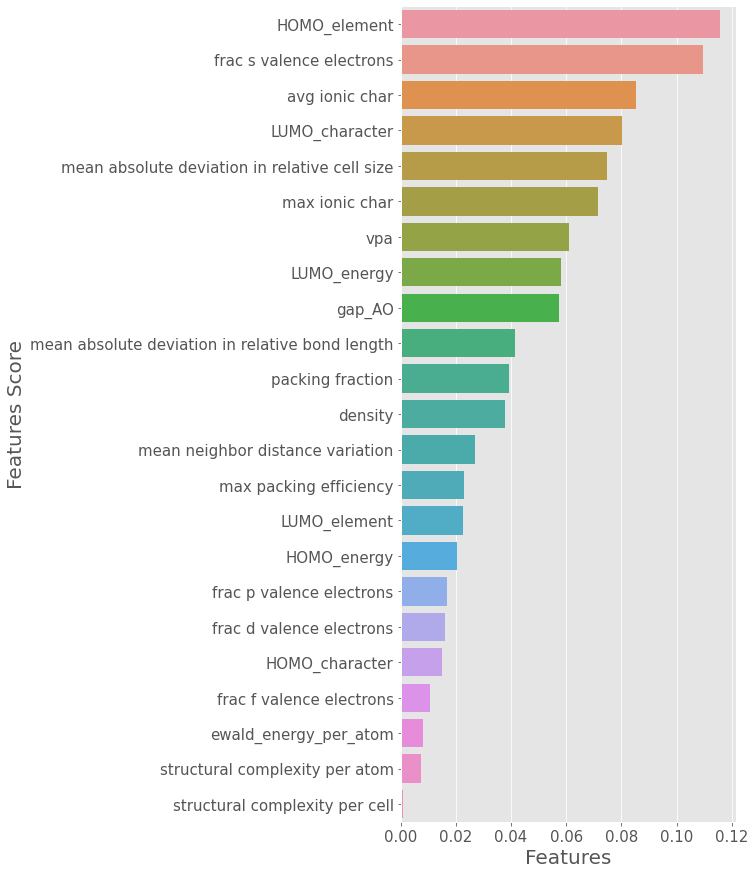
\includegraphics[width=3in]{Figures/Heuslers_FI.png}  
        \label{fig:MLmodel_Heuslers_FI}
        }
        \quad
        \subfigure[]
        {
        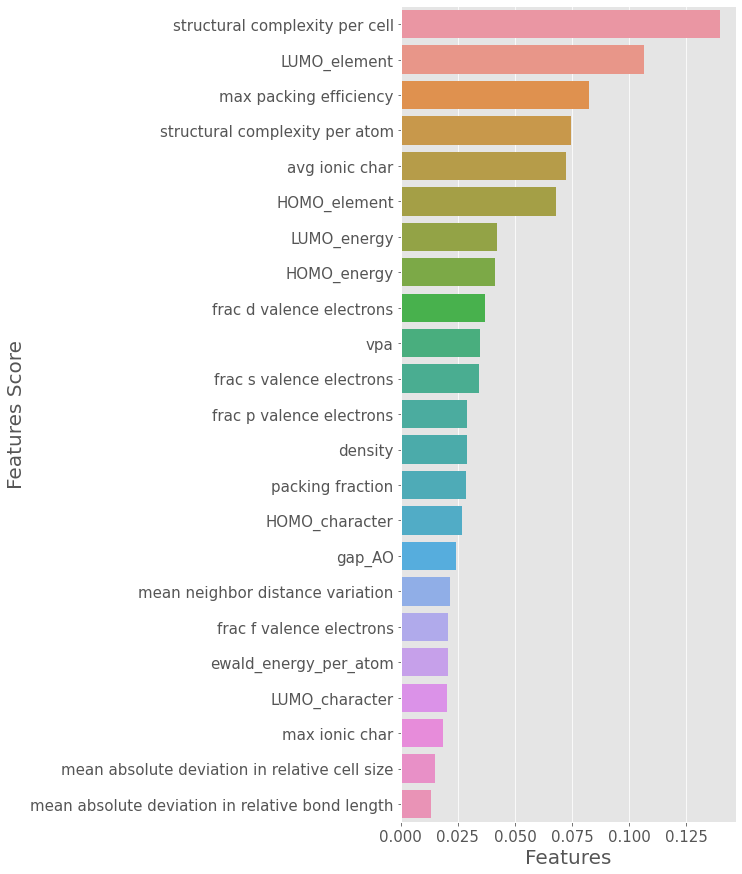
\includegraphics[width=3in]{Figures/Cubic_FI.png}  
        \label{fig:MLmodel_Cubic_FI}
        }
\caption{a) Feature important scoring (Gain) for a) Heuslers compounds ML model, and b) Cubic compounds ML model. [Colors online]}
\label{fig:MLmodelFI}
\end{figure}

%\section{Discussion}
%This section will tentatively discuss: 
%\begin{enumerate}
%    \item how similar/dissimilar could be the performances for ML and GNN models Mentioning the possible root cause.
%    \item how 
%\end{enumerate}

\section{Conclusions}
In this work, we used machine learning to develop a model correlating composition vs. number of Dirac points (called the number of crossings) in the electronic band structures for Heuslers and other Cubic compounds by identifying said crossings using an automated algorithm as well as generating chemical composition and global crystal structure features. In general, our ML model captured the overall trend in the Heuslers, predicting the EBS number of crossings; however, the ML model (parity plot) suffered from  significant variance. The Heuslers datasets size (\num{276} compounds) was not the limiting factor in regards of the variance; an additional ML model was created for the larger dataset of Cubic compounds of size ($\sim$\num{3800} compounds), and it also exhibited a similar variance. This is, however, within expectation, due to the nature of the EBS where it is well understood that atomic site specific properties determine the band structure. A methodology for handling atomic site specific features has to be developed such that ML models can incorporate their description, in a better match to the underlying quantum mechanics governing the properties, and capture the electronic properties in a more generalized approach. This atomic site specific approach is, however, difficult due to the feature dimensionality dramatically increasing as, for example, the number of possible atomic sites (up to 64) convolved with the number of possible elements at each site (up to 118) convolved with the number of atomic orbitals at each site (up to 14), becomes unuseably large. Thus, an open challenge for future applications of ML in electronic materials intelligence, requires the development of featurizers that are able to generate atomic site features but also encoding them into artificial structural features to reduce the dimensionality.

%Our ML model identified electronic properties related to the HOMO-LUMO frontier energy levels, and structural complexity based on \textcolor{red}{XXX and XXX}. which could better describe/capture site-specific physic.

%\section{Bibliography styles}
%There are various bibliography styles available. You can %select the style of your choice in the preamble of this document. These styles are Elsevier styles based on standard styles like Harvard and Vancouver. Please use Bib\TeX\ to generate your bibliography and include DOIs whenever available.
%Here are two sample references: \cite{Feynman1963118,Dirac1953888}.

\bibliography{mybibfile}

\end{document}
